% ---------- Titelblad Masterproef Faculteit Wetenschappen -----------
% Dit document is opgesteld voor compilatie met pdflatex.  Indien je
% wilt compileren met latex naar dvi/ps, dien je de figuren naar
% (e)ps-formaat om te zetten.
%                           -- december 2012
% -------------------------------------------------------------------
\RequirePackage{fix-cm}
\documentclass[12pt,a4paper,oneside]{article}

% --------------------- In te laden pakketten -----------------------
% Deze kan je eventueel toevoegen aan de pakketten die je al inlaadt
% als je dit titelblad integreert met de rest van thesis.
% -------------------------------------------------------------------
\usepackage{graphicx,xcolor,textpos}
\usepackage{helvet}

% -------------------- Pagina-instellingen --------------------------
% Indien je deze wijzigt, zal het titelblad ook wijzigen.  Dit dien je
% dan manueel aan te passen.
% --------------------------------------------------------------------

\topmargin -10mm
\textwidth 160truemm
\textheight 240truemm
\oddsidemargin 0mm
\evensidemargin 0mm

% ------------------- textpos-instellingen ---------------------------
% Enkele andere instellingen voor het voorblad.
% --------------------------------------------------------------------

\definecolor{green}{RGB}{172,196,0}
\definecolor{bluetitle}{RGB}{29,141,176}
\definecolor{blueaff}{RGB}{0,0,128}
\definecolor{blueline}{RGB}{82,189,236}
\setlength{\TPHorizModule}{1mm}
\setlength{\TPVertModule}{1mm}



%----------------------- Custom stuff -------------------------------

\graphicspath{./}
\usepackage{makeidx}
\index{hoofd}
\makeindex
\usepackage{amsmath}
\usepackage[dutch]{babel}

\usepackage{hyperref}
\usepackage{graphicx}
\usepackage{caption}
\usepackage{subcaption}




%------------------------ Plot packages ----------------------------
\usepackage{tikz}
\usepackage{pgfplots}

\usepackage{pgf}
\usepackage{units}
\usepackage{metalogo}







% --------------------------------------------------------------------


\title{Project wavelets}
\author{Matthias Baeten \& Bob Vergauwen}
\date{ 13 januari 2016}

\begin{document}

\maketitle

\section{Ruisreductie}

\subsection{Academisch voorbeeld zonder ruis}

Bij wijze van opwarming starten we met de wavelet decompositie van de functie $ \mathbb{R}  \to \mathbb{R}: x \mapsto \exp(x)$. 
Dit is een gladde functie die bovendien analytisch is. 
Voor onze analyse werden de de exponenti\"ele functie equidistant bemonster op het interval $ [0,1] $ met $ 256 $ punten.
Deze data werd nadien geanalyseerd met behulp van 3 verschillende wavelet transformaties, de haar wavelet, de daubechie wavelet van orde 4 en de daubechie wavelet van orde 45.
Elk van deze transformaties werd uitgevoerd tot niveau 4, dit maakt dus dat het signaal zal worden opgesplitst ten opzichte van 5 verschillende basissen.  
De resultaten van dit experiment zijn samen gevat in Figuur \ref{fig:exp_noNoise}.
In de linker kolom van de figuur zijn de coefficienten van de transformatie uitgezet.
In de rechter kolom is telkens de benadering van de exponenti\"ele functie in elke basis uitgezet.
Hierbij is de onderste curve de benadering in $ W_1 $, die daar boven de benadering in $ W_2 $ en zo voort.
De bovenste grafiek is dan de benardering van de exponenti\"ele functie in de ruimte $ V_4 $.

Wat meteen opvalt is dat de coefficienten van de lage frequenties (links in de coefficienten vector) het grootst zijn.
Dit is volledig volgens de verwachting, de exponentiele funtie is een gladde functie en bevat dus voornamelijk lage frequenties.
Een tweede bemerking is dat voor de hogere orde wavelets de coefficienten aan de randen groter worden.
Dit is het gevolg van het breder worden van de wavelet, hierdoor zal het eind effect verstrekt worden.

Vervolgens kunnen we zien naar de kwaliteit van de benaderingen in de opeen volgde vector ruimtes, zoals gegeven in de rechter kolom.
Hier is het duidelijk dat een hogere orde benadering niet meteen een snellere convergentie geeft.
Dit is opnieuw het gevolg van het bredere karakter van de hogere orde wavelets.
Over het algemeen is de beste benadering bekomen door de daubechie wavelte van orde 2.
Het eind effect is het kleinste voor de haar wavelet.

\subsection{Academisch voorbeeld met ruis}

In een tweede test word er ruis toegevoegd aan de gladde functie exponenti\"ele functie.
Deze ruis is witte ruis met een standaard afwijking van 0.1.
Om de invloed van de ruis op de wavelet coefficienten duidelijk te maken zijn de coefficienten weergegeven in 
figuur \ref{fig:exp_Noise_noise_10}.
De invloed van de witte ruis in het tijddomein geeft  een verstoring van witte ruis op de coefficienten van de versrchillende wavelet transformaties.
De verstoring kan makkelijk worden verwijderd aan de hand van een treshold waarder te gebruiken.
Deze methode is besproken in de opgaven en zal dus niet verder worden toegelicht.
Enkel de resultaten en toepassingen zullen worden besproken.

De fout als functie van de threshold waarden is weergeven in figuur \ref{fig:error_exp_haar_10} tot \ref{fig:error_exp_db45_10}.
Uit deze drie figuren is het duidelijk dat er een fundamenteel verschil optreed tussen de zachte threshold functie en de twee andere.
De verklaring hiervoor is dat de zachte threshold functie elke waarden zal wijzigen, zelfs de waarden ver boven de threshold.
Om dit te illustreren zijn de drie threshold functies weergegeven in Figuur \ref{fig:Threshold}.

Om dit deel af te sluiten is in figuur \ref{fig:Optimale_ruisReductie} de optimale ruis reductie weergegeven.
Deze reducties maakt gebruik van daubechie wavelet van orde 2 en een threshold waarden van 0.4 met  de zachte treshold functie.


\paragraph{Tussenliggende waarden bepalen}

\dots Iets met de basis wavelet bepalen in het punt  en zo kan je het doen. Ik denk dat dit iets te maken heeft met een wavelet interpolatie.









\begin{figure}
    \centering
     \begin{subfigure}[b]{0.45\textwidth}
            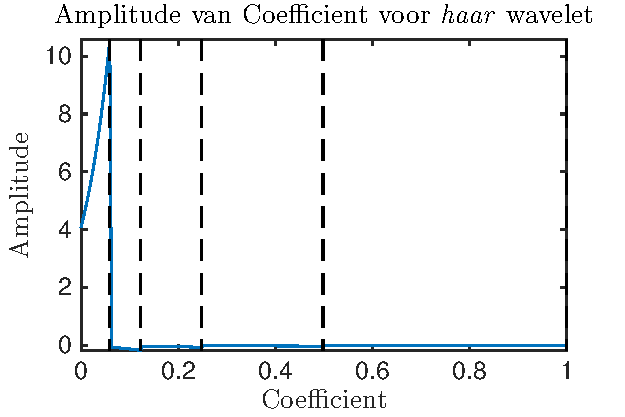
\includegraphics[width=\textwidth]{../src/denoising/haar_noNoise/coef_exp_haar_4}
            \caption{Met tekst beschadiging}
            \label{fig:tiger}
        \end{subfigure}
        ~ %add desired spacing between images, e. g. ~, \quad, \qquad, \hfill etc. 
        %(or a blank line to force the subfigure onto a new line)
        \begin{subfigure}[b]{0.45\textwidth}
            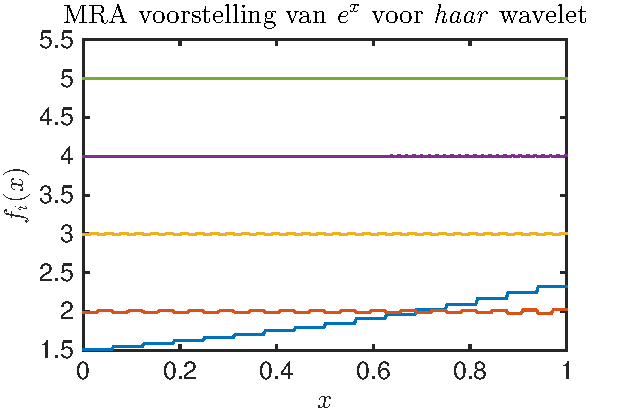
\includegraphics[width=\textwidth]{../src/denoising/haar_noNoise/MRA_exp_haar_4}
            \caption{Na de reconstructie}
            \label{fig:mouse}
        \end{subfigure}
    \begin{subfigure}[b]{0.45\textwidth}
        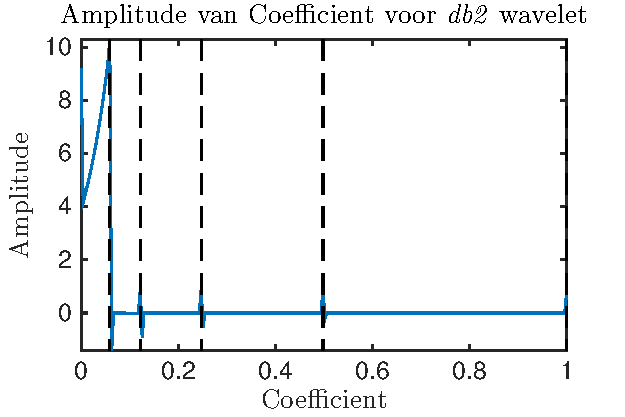
\includegraphics[width=\textwidth]{../src/denoising/db2_noNoise/coef_exp_db2_4}
        \caption{Met tekst beschadiging}
        \label{fig:tiger}
    \end{subfigure}
    ~ %add desired spacing between images, e. g. ~, \quad, \qquad, \hfill etc. 
    %(or a blank line to force the subfigure onto a new line)
    \begin{subfigure}[b]{0.45\textwidth}
        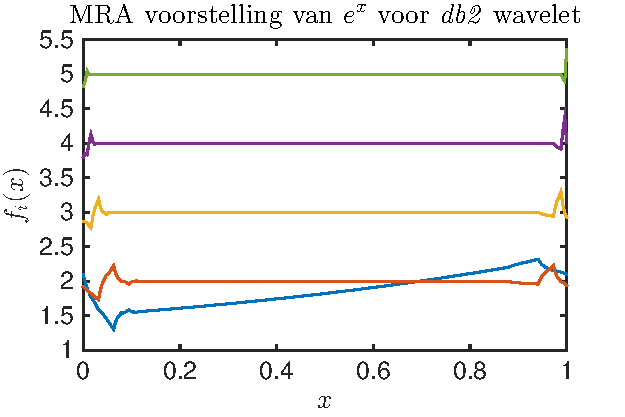
\includegraphics[width=\textwidth]{../src/denoising/db2_noNoise/MRA_exp_db2_4}
        \caption{Na de reconstructie}
        \label{fig:mouse}
    \end{subfigure}
    \begin{subfigure}[b]{0.45\textwidth}
        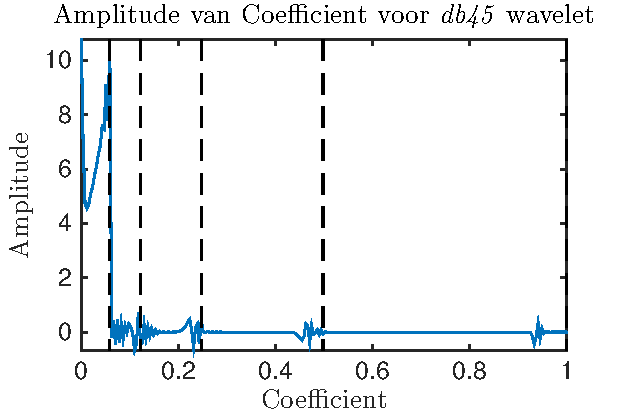
\includegraphics[width=\textwidth]{../src/denoising/db45_noNoise/coef_exp_db45_4}
        \caption{Met tekst beschadiging}
        \label{fig:tiger}
    \end{subfigure}
    ~ %add desired spacing between images, e. g. ~, \quad, \qquad, \hfill etc. 
    %(or a blank line to force the subfigure onto a new line)
    \begin{subfigure}[b]{0.45\textwidth}
        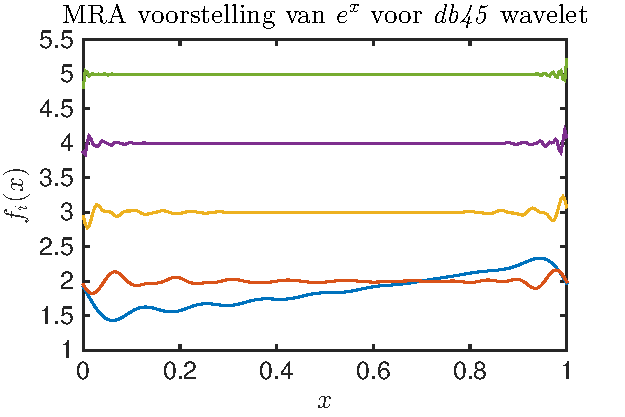
\includegraphics[width=\textwidth]{../src/denoising/db45_noNoise/MRA_exp_db45_4}
        \caption{Na de reconstructie}
        \label{fig:mouse}
    \end{subfigure}
    \caption{Pictures of lena}\label{fig:exp_noNoise}
\end{figure}






\begin{figure}
    \centering
     \begin{subfigure}[b]{0.45\textwidth}
            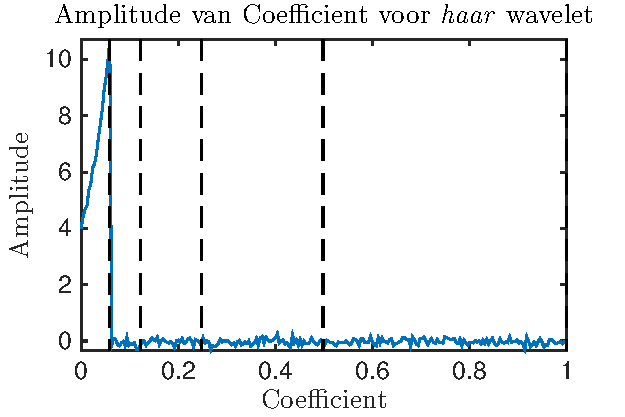
\includegraphics[width=\textwidth]{../src/denoising/haar_Noise/coef_exp_haar_4_noise_10}
            \caption{Met tekst beschadiging}
            \label{fig:tiger}
        \end{subfigure}
        ~ %add desired spacing between images, e. g. ~, \quad, \qquad, \hfill etc. 
        %(or a blank line to force the subfigure onto a new line)
        \begin{subfigure}[b]{0.45\textwidth}
            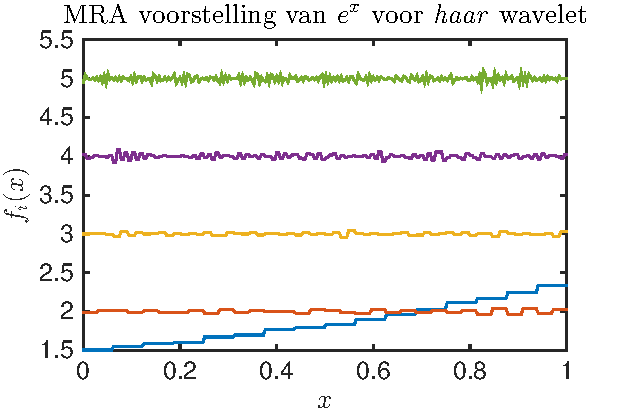
\includegraphics[width=\textwidth]{../src/denoising/haar_Noise/MRA_exp_haar_4_noise_10}
            \caption{Na de reconstructie}
            \label{fig:mouse}
        \end{subfigure}
    \begin{subfigure}[b]{0.45\textwidth}
        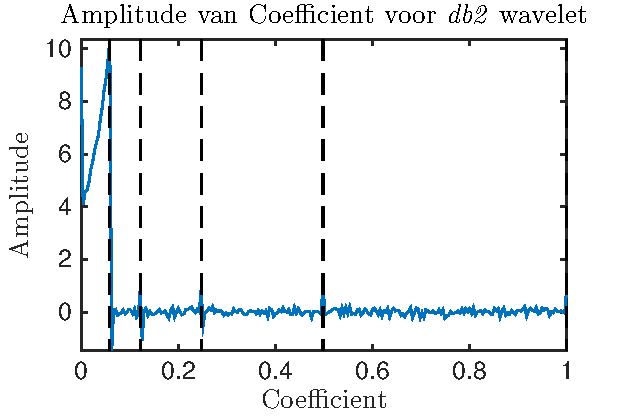
\includegraphics[width=\textwidth]{../src/denoising/db2_Noise/coef_exp_db2_4_noise_10}
        \caption{Met tekst beschadiging}
        \label{fig:tiger}
    \end{subfigure}
    ~ %add desired spacing between images, e. g. ~, \quad, \qquad, \hfill etc. 
    %(or a blank line to force the subfigure onto a new line)
    \begin{subfigure}[b]{0.45\textwidth}
        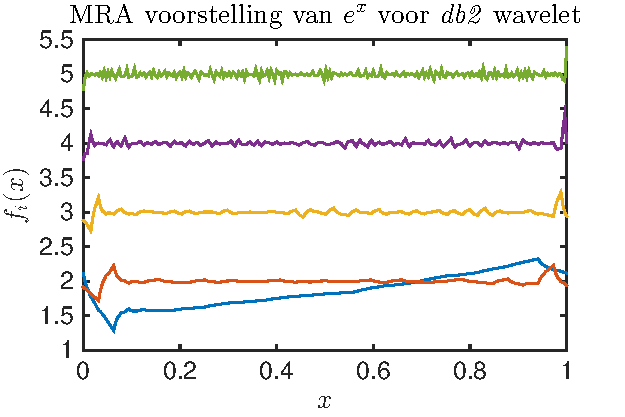
\includegraphics[width=\textwidth]{../src/denoising/db2_Noise/MRA_exp_db2_4_noise_10}
        \caption{Na de reconstructie}
        \label{fig:mouse}
    \end{subfigure}
    \begin{subfigure}[b]{0.45\textwidth}
        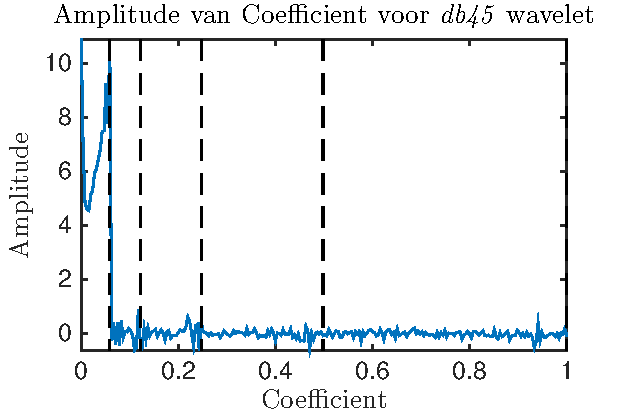
\includegraphics[width=\textwidth]{../src/denoising/db45_Noise/coef_exp_db45_4_noise_10}
        \caption{Met tekst beschadiging}
        \label{fig:tiger}
    \end{subfigure}
    ~ %add desired spacing between images, e. g. ~, \quad, \qquad, \hfill etc. 
    %(or a blank line to force the subfigure onto a new line)
    \begin{subfigure}[b]{0.45\textwidth}
        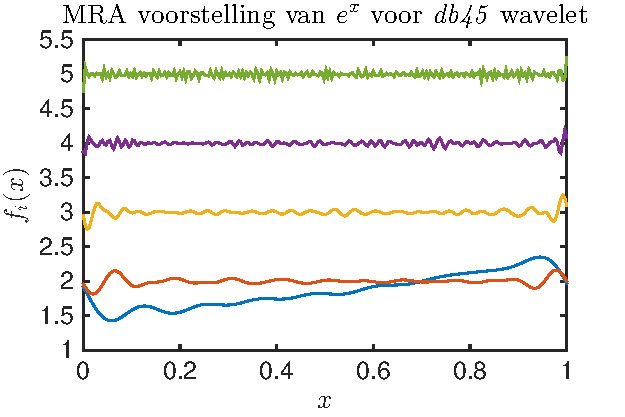
\includegraphics[width=\textwidth]{../src/denoising/db45_Noise/MRA_exp_db45_4_noise_10}
        \caption{Na de reconstructie}
        \label{fig:mouse}
    \end{subfigure}
    \caption{Pictures of lena}\label{fig:exp_Noise_noise_10}
\end{figure}






\begin{figure}
\centering
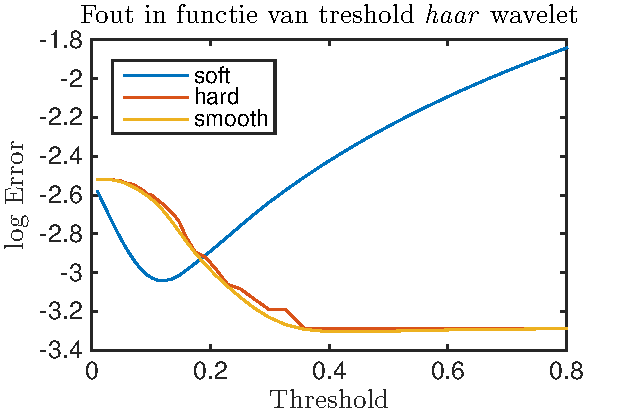
\includegraphics[width=0.7\linewidth]{../src/denoising/error_1d/error_exp_haar_10}
\caption{}
\label{fig:error_exp_haar_10}
\end{figure}
\begin{figure}
\centering
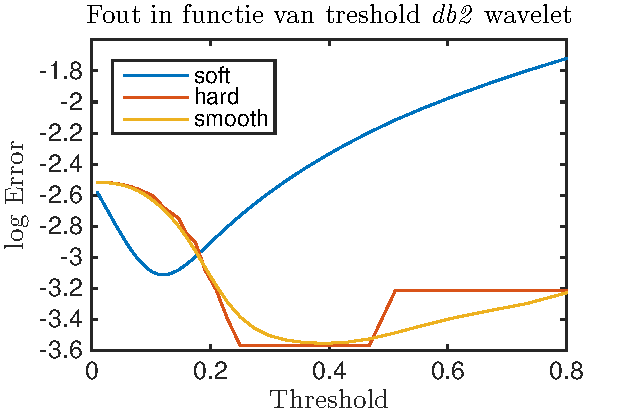
\includegraphics[width=0.7\linewidth]{../src/denoising/error_1d/error_exp_db2_10}
\caption{}
\label{fig:error_exp_db2_10}
\end{figure}
\begin{figure}
\centering
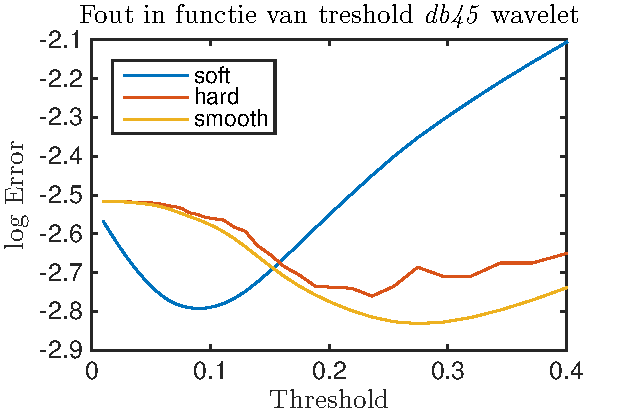
\includegraphics[width=0.7\linewidth]{../src/denoising/error_1d/error_exp_db45_10}
\caption{}
\label{fig:error_exp_db45_10}
\end{figure}


\begin{figure}
\centering
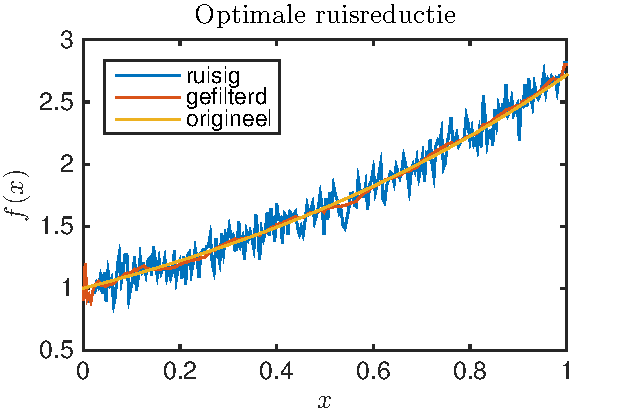
\includegraphics[width=0.7\linewidth]{../src/denoising/error_1d/Optimale_ruisReductie}
\caption{}
\label{fig:Optimale_ruisReductie}
\end{figure}

\begin{figure}
\centering
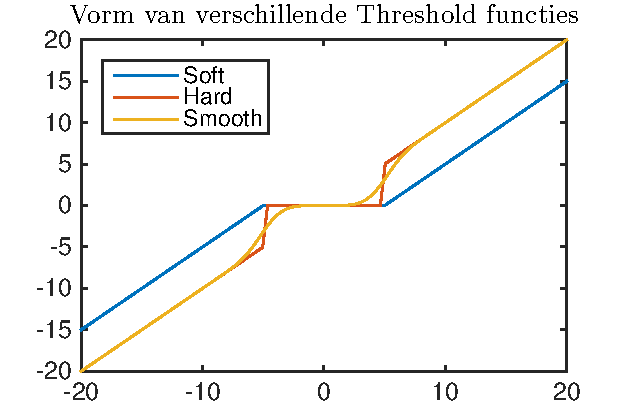
\includegraphics[width=0.7\linewidth]{../src/denoising/error_1d/Threshold}
\caption{}
\label{fig:Threshold}
\end{figure}






\subsection{Moving on to images}

\subsubsection{Implementatie van ruis reductie algoritme}


De eenvoudigste manier voor ruis uit een afbeelding te halen aan de hand van een wavelet transformatie is door exact de zelfde strategie toe te passen als in het 1 dimensionaal geval.
Dit houd in dat eerst de wavelet coefficienten worden bepaald voor de ruisige afbeelding.
Nadien worden deze coefficienten met een threshold functie op een niet lineaire manier gefilterd.
De laatste stap is dan de afbeelding reconstrueren aan de hand van de gefilterde coefficienten.
Een concrete implementatie van dit algoritme is terug te vinden in de appendix.

\subsubsection{Verschil in threshold functies}

Voor een goed beeld te krijgen van de invloed van de threshold functie op de ruisreductie hebben we de kwaliteit van de ruisreductie vergeleken voor de verschillende threshold functies.
Voor elke threshold functie werden er een aantal threshold parameters getest.
Een voorbeeld resultaat van zo een test is te zien in Figuur \ref{fig:snr_image_bior6}.
Uit deze afbeelding is af te leiden dat zachte threshold functie het beste resultaat opleverd voor de ruisreductie.
In Figuur \ref{fig:snr_image_bior6} werd gebruik gemaakt van de biorthogonale wavelet van orde 6,8.
Voor de meeste andere transformaties werden gelijkaardige resultaten bekomen.
We kunnen dus besluiten dat de zachte threshold functie de beste ruisreductie oplevert.


\begin{figure}
\centering
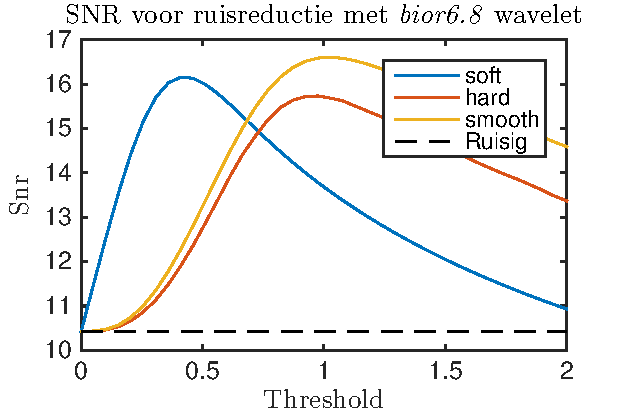
\includegraphics[width=0.7\linewidth]{../src/denoising/image/snr_image_bior68_30.pdf}
\caption{}
\label{fig:snr_image_bior6}
\end{figure}


\subsubsection{Optimale threshold bepalen(met vals spelen)}

Uit het vorige experiment hebben we kunnen besluiten dat in alle gevallen de zachte threshold functie de beste denoising geeft.
Een tweede resultaat dat opviel was dat de SNR curves steeds vlakke curves bleken te zijn voor de zachte threshold functie.
Door het gladde karakter van deze curve is het gebruik van een optimalisatie routine voor de SNR costfunctie makkelijk te implementeren.
De cost functie is als volgt gedefini\"eerd in matlab.
\begin{verbatim}
costFun = @(delta) -snr_denoising(mode, thres, delta, wname, ...
                   Nb_levels, A_origineel, A_noise,0);
\end{verbatim}
Dit is een functie in de parameter \verb|delta|. Dit is de waarden van de threshold.
Merk op dat voor de berekening van de SNR waarden de originele afbeelding moet gekend zijn. (Vals spelen dus)
Door gebruik te maken van \verb|fmincon| is de keuze van de optimale parameter eenvoudig gemaakt.

Een voorbeeld resultaat van de optimale ruis onderdrukking is gegeven in figuur \ref{fig:optimaleRuisBIOR}.
In deze figuur is opnieuw de biorthogonale wavelet van orde 6,8 gebruikt.


\begin{figure}
    \centering
    \begin{subfigure}[b]{0.45\textwidth}
        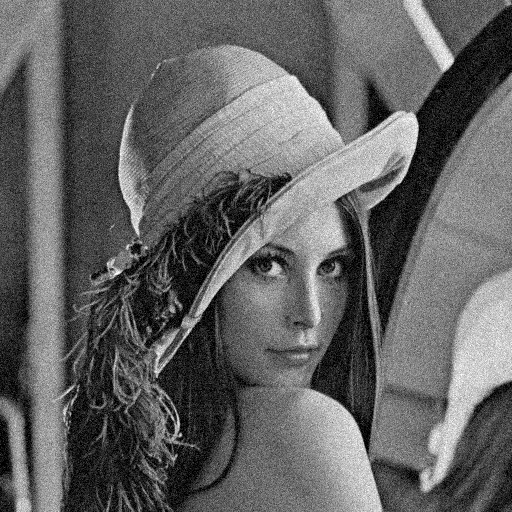
\includegraphics[width=\textwidth]{../src/denoising/image/lenaNoise_bior68.png}
        \caption{Met tekst beschadiging}
        \label{fig:tiger}
    \end{subfigure}
    ~ %add desired spacing between images, e. g. ~, \quad, \qquad, \hfill etc. 
    %(or a blank line to force the subfigure onto a new line)
    \begin{subfigure}[b]{0.45\textwidth}
        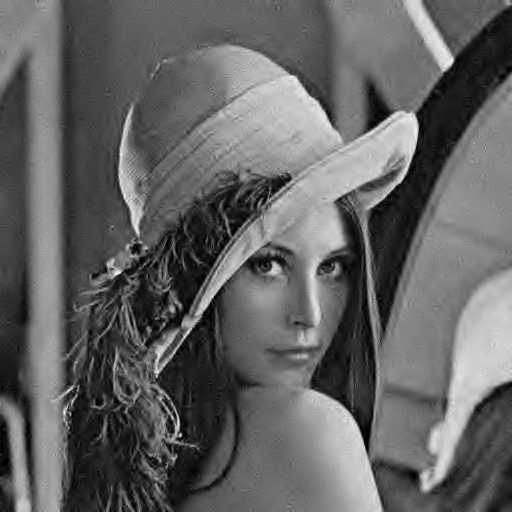
\includegraphics[width=\textwidth]{../src/denoising/image/lenaDen_bior68.png}
        \caption{Na de reconstructie}
        \label{fig:mouse}
    \end{subfigure}
    \caption{Pictures of lena}\label{fig:optimaleRuisBIOR}
\end{figure}


\subsubsection{Optimale threshold bepalen(zonder vals spelen)}




\section{Inpainting}

In dit hoofdstuk zullen we wavelets gebruiken om ontbrekende regio's in foto's in te kleuren. Deze methode wordt gebruikt om beschadigde foto's te reconstrueren. De schade op de foto wordt gemodelleerd met pixel waarden in de foto die verdwenen zijn. Om de verdwenen regio's in te kleuren wordt de iteratieve methode gebruikt die beschreven staat in de opgave. We hebben dit algoritme ge\"{i}mplementeerd in Matlab met behulp van de Wavelet toolbox. Hierbij nemen we een bepaalde foto en verwijderen we de pixels in bepaalde regio's. Het algoritme probeert dan de verdwenen regio's in te kleuren. 
\newline
\newline
In figuur \ref{fig:matti_fig_1} wordt het algoritme ge\"{i}llustreerd met verschillende soorten regio's van pixels die verwijderd zijn. In figure \ref{fig:matti_fig_1a} zijn er blokken pixels verwijderd, in figuur \ref{fig:matti_fig_1c} zijn er random pixels verwijderd en in figuur \ref{fig:matti_fig_1e} is de figuur overschreven met tekst. De resultaten van het 'inpainting' algoritme staan er steeds naast. Het algoritme geeft op het eerste zicht heel mooie resultaten. Alleen als we de ingekleurde resultaten in detail gaan bekijken merken we dat het niet de originele figuren zijn. Dit is het meest duidelijk bij de figuren die bewerkt zijn met blokken en met tekst.
\newline
\newline
Het 'inpainting' algoritme kan gebruikt worden op verschillende manieren. Zo zijn er verschillende soorten wavelets die gebruikt kunnen worden. De thresholding kan op verschillende manieren gebeuren en de threshold parameter $\delta$ moet gekozen worden. De effecten op het resultaat van al deze verschillende soorten instellingen zullen besproken worden in de volgende hoofdstukken.

\begin{figure}
    \centering
    \begin{subfigure}[b]{0.45\textwidth}
        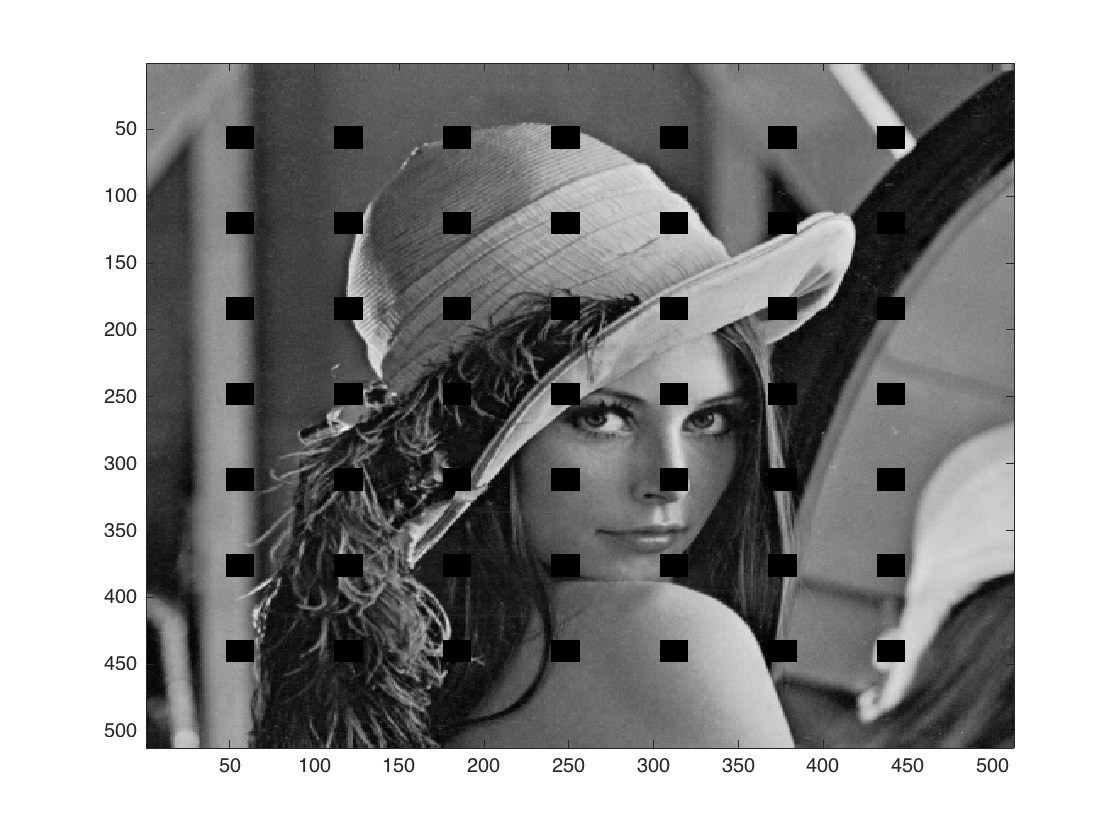
\includegraphics[width=\textwidth]{../src/inpainting/lena_block}
        \caption{Foto van Lena met vierkante blokjes pixels verwijderd (zwart gemaakt). }
        \label{fig:matti_fig_1a}
    \end{subfigure}
    ~ %add desired spacing between images, e. g. ~, \quad, \qquad, \hfill etc. 
    %(or a blank line to force the subfigure onto a new line)
    \begin{subfigure}[b]{0.45\textwidth}
        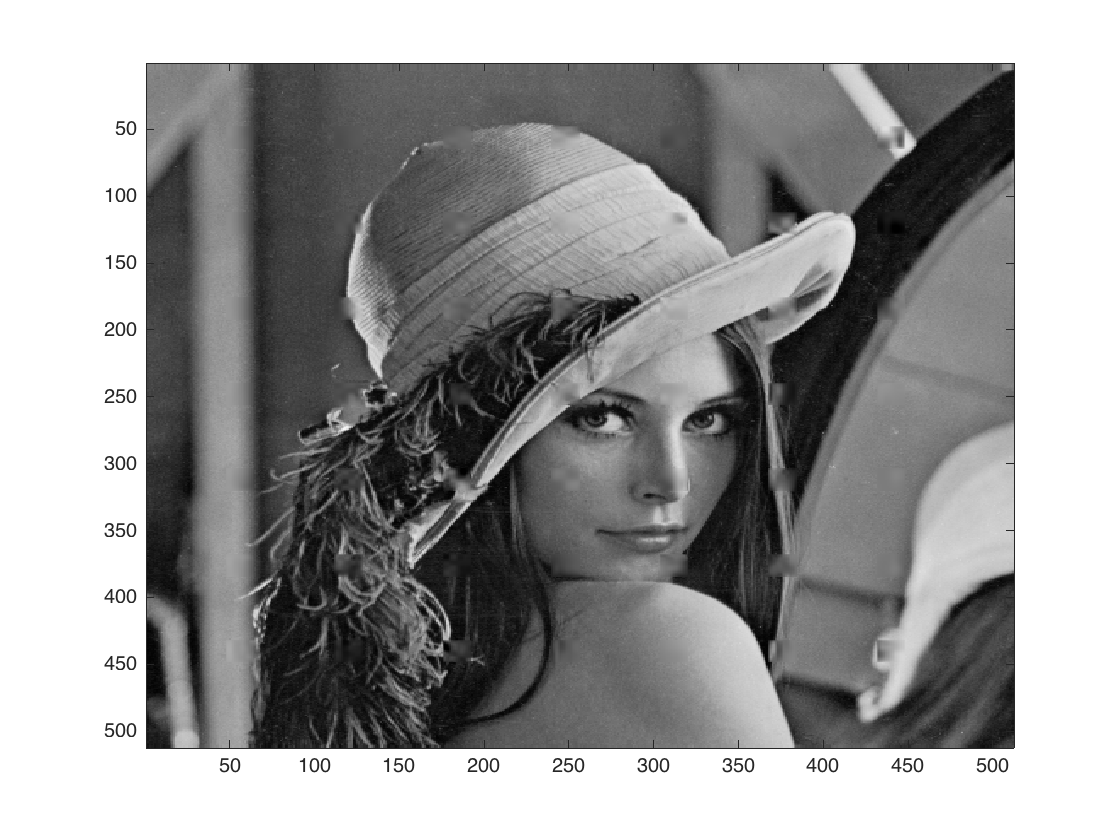
\includegraphics[width=\textwidth]{../src/inpainting/lena_blok_painted_1}
        \caption{Foto \ref{fig:matti_fig_1a} ingekleurd. \\ \ \\}
        \label{fig:matti_fig_1b}
    \end{subfigure}
    \begin{subfigure}[b]{0.45\textwidth}
        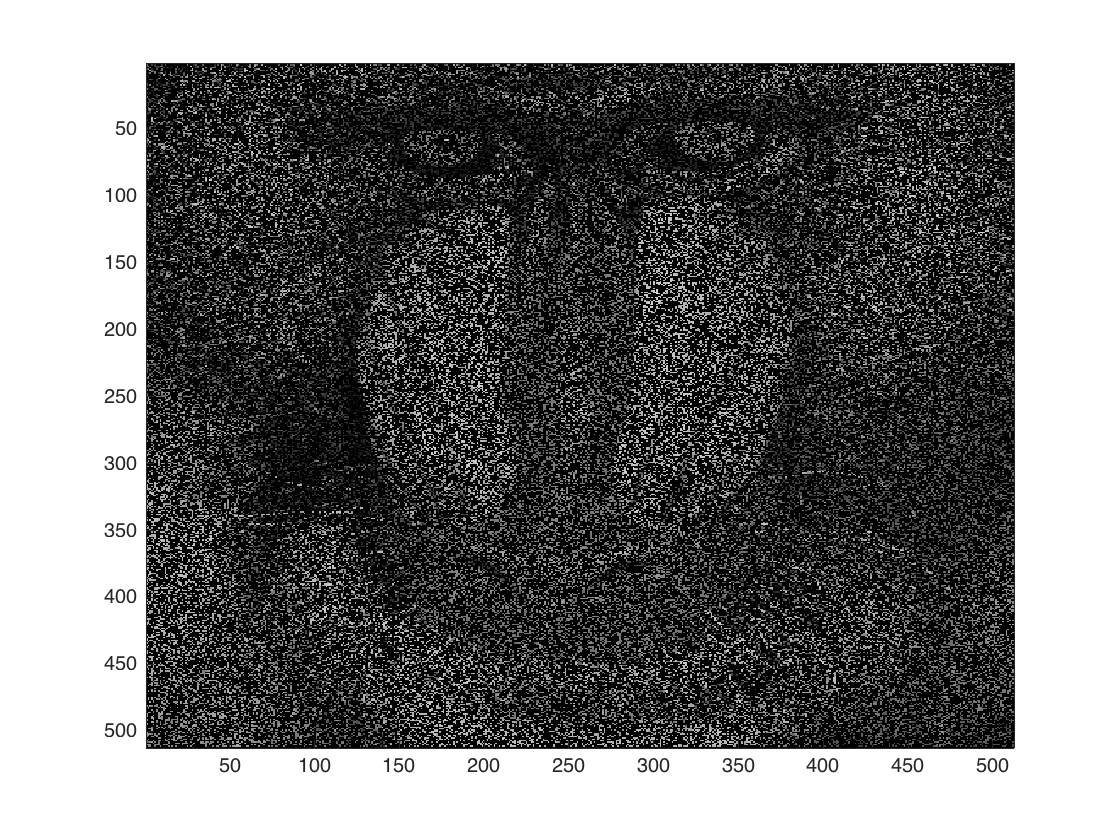
\includegraphics[width=\textwidth]{../src/inpainting/baboon_random_noise_1}
        \caption{Foto van aap met ongeveer 70 procent van de pixels verwijderd (zwart gemaakt). }
        \label{fig:matti_fig_1c}
    \end{subfigure}
    ~ %add desired spacing between images, e. g. ~, \quad, \qquad, \hfill etc. 
    %(or a blank line to force the subfigure onto a new line)
    \begin{subfigure}[b]{0.45\textwidth}
        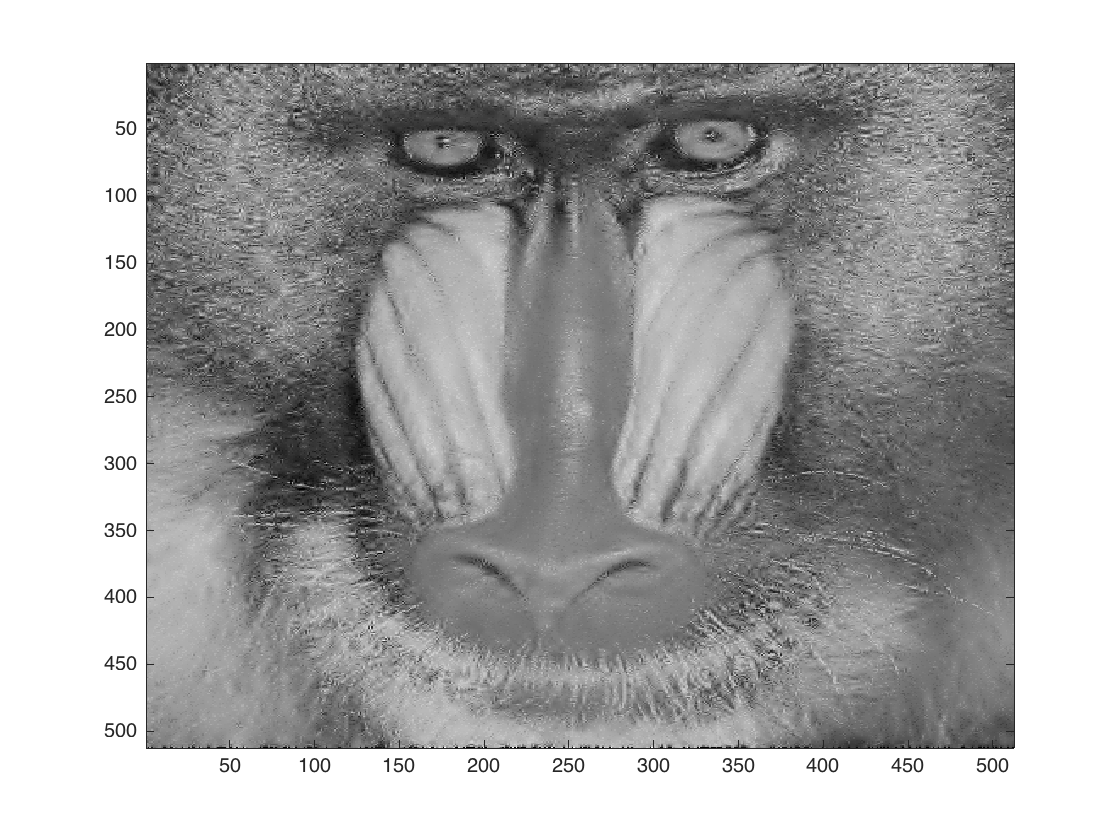
\includegraphics[width=\textwidth]{../src/inpainting/baboon_random_fixed_1}
        \caption{Foto \ref{fig:matti_fig_1c} ingekleurd. \\ \ \\}
        \label{fig:matti_fig_1d}
    \end{subfigure}
        \begin{subfigure}[b]{0.45\textwidth}
        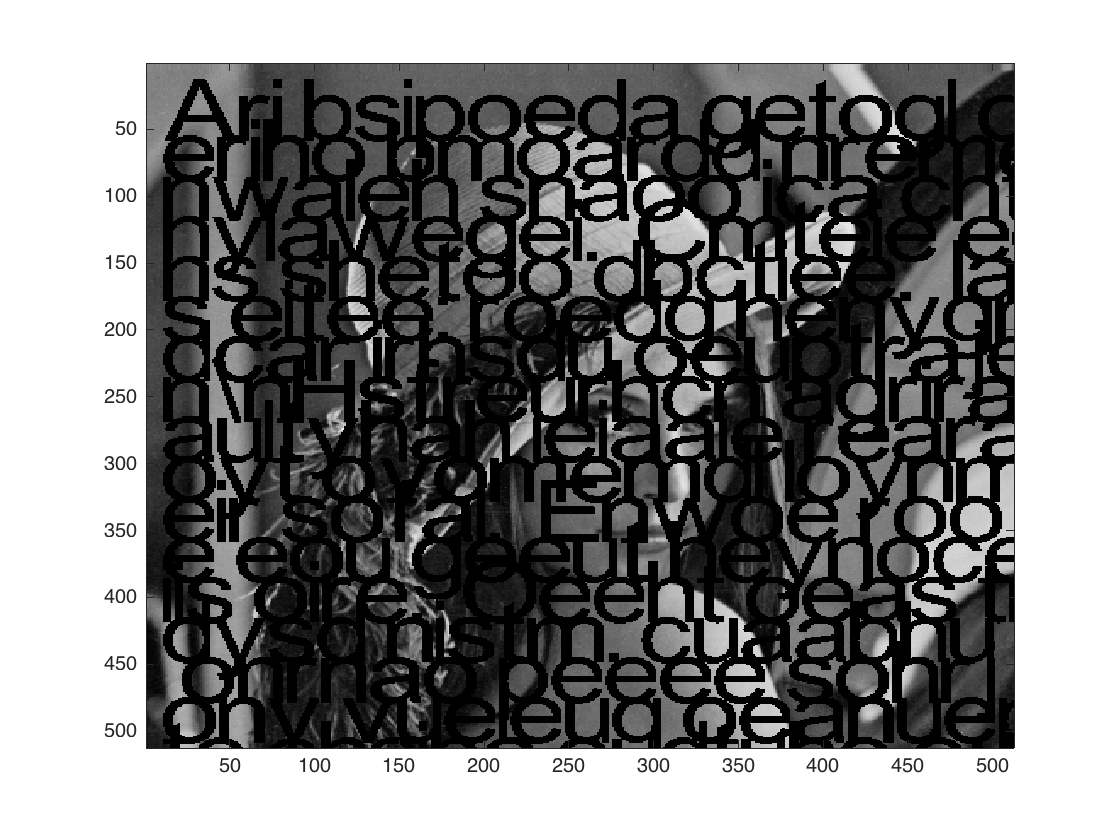
\includegraphics[width=\textwidth]{../src/inpainting/lena_letters_broke_1}
        \caption{Foto van lena overschreven met tekst. }
        \label{fig:matti_fig_1e}
    \end{subfigure}
    ~ %add desired spacing between images, e. g. ~, \quad, \qquad, \hfill etc. 
    %(or a blank line to force the subfigure onto a new line)
    \begin{subfigure}[b]{0.45\textwidth}
        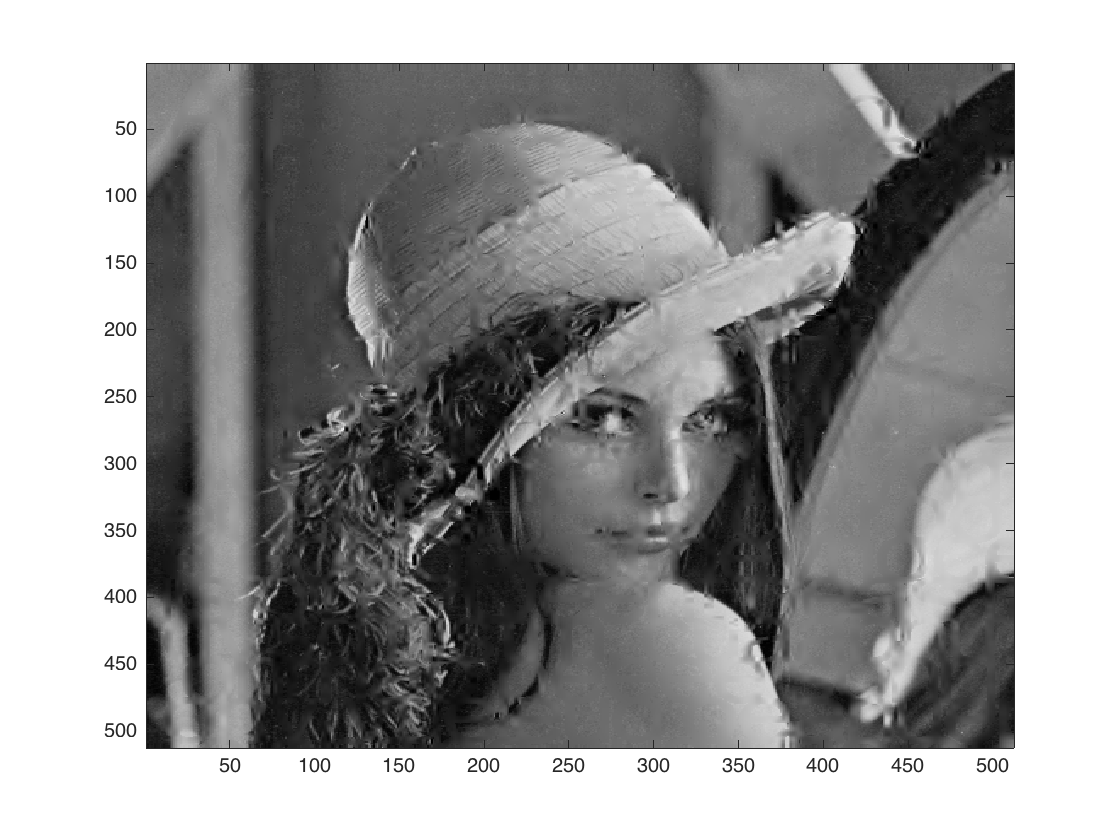
\includegraphics[width=\textwidth]{../src/inpainting/lena_letters_fixed_1}
        \caption{Foto \ref{fig:matti_fig_1e} ingekleurd.}
        \label{fig:matti_fig_1f}
    \end{subfigure}
    \caption{Resultaten van het 'Inpainting' algoritme. Instellingen algoritme: wavelet: 'db5', level $N = 10$, soft thresholding, threshold parameter $\delta = 10$, 200 iteraties.}\label{fig:matti_fig_1}
\end{figure}

\FloatBarrier


\subsection{Threshold technieken}

\begin{figure}[!]
    \centering
    \begin{subfigure}[b]{0.45\textwidth}
        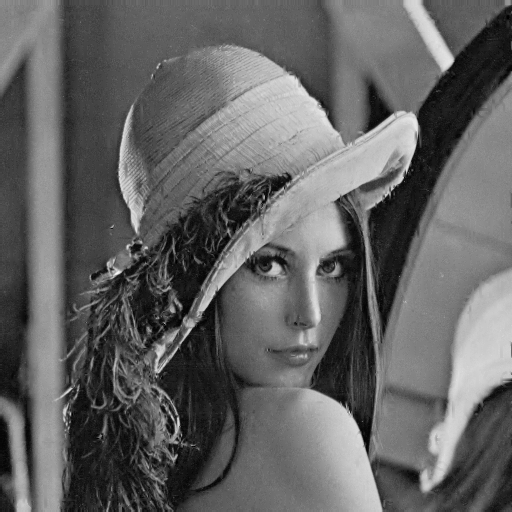
\includegraphics[width=\textwidth]{../src/inpainting/lena_soft_2}
        \caption{ \textbf{Soft thresholding ($\mathbf{\delta = 10 }$)}.}
        \label{fig:matti_soft_2}
    \end{subfigure}
    ~ %add desired spacing between images, e. g. ~, \quad, \qquad, \hfill etc. 
    %(or a blank line to force the subfigure onto a new line)
    \begin{subfigure}[b]{0.45\textwidth}
        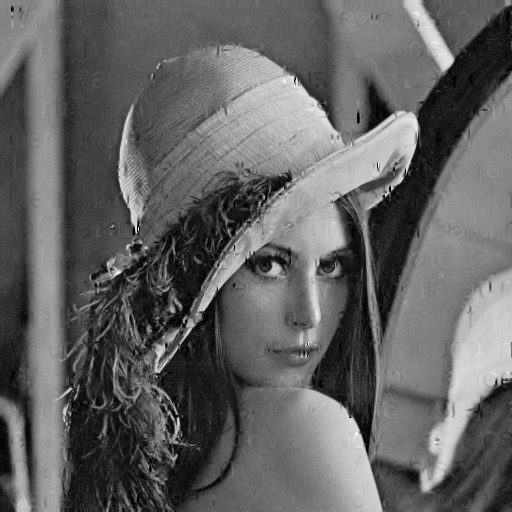
\includegraphics[width=\textwidth]{../src/inpainting/lena_hard_2}
        \caption{ \textbf{Hard thresholding ($\mathbf{\delta = 100 }$)}.}
        \label{fig:matti_hard_2}
    \end{subfigure}
    \caption{Met tekst overschreven figuur \ref{fig:matti_fig_1e} ingekleurd met 'inpainting' algoritme. Instellingen algoritme: wavelet: 'db5', level $N = 10$, 200 iteraties.}\label{fig:matti_hardsoft}
\end{figure}

\FloatBarrier


Er zijn 2 soorten technieken voor thresholding, namelijk soft thresholding en hard thresholding. Voor beide technieken moet ook een threshold parameter $\delta > 0$ gekozen worden. In figuur \ref{fig:matti_hardsoft} is een figuur ingekleurd op twee manieren. E\'{e}n keer met soft thresholding en threshold parameter $\delta = 10$ en de andere keer met hard thresholding en threshold parameter $\delta = 100$. In het geval van soft thresholding was het gemakkelijk om een threshold parameter te vinden die redelijk goede resultaten geeft. Voor hard thresholding was het langer zoeken achter een geschikte threshold parameter $\delta = 100$. Dit was de meest optimale waarde van $\delta$ die ik op het eerste zicht kon vinden. Het is duidelijk dat voor soft thresholding betere resultaten kunnen bekomen worden als voor hard thresholding. Bij hard thresholding zijn er nog veel randen van letters zichtbaar. Bij soft thresholding zijn de resultaten veel beter. 
\newline
\newline
Het is duidelijk dat het vinden van de optimale threshold parameter $\delta$ zo eenvoudig is. Daarom zullen we het volgende experiment uitvoeren. We voeren het 'inpainting' algoritme uit voor een reeks van verschillende waardes van $\delta$. Voor elke waarde van $\delta$ zal het relatieve verschil tussen de ingekleurde foto en de originele onbeschadigde foto berekent worden. Dit verschil wordt voorgesteld op de volgende manier:

\begin{equation} \label{eq:matti_eq1}
\frac{\left\lVert A_{\text{ingekleurd}} - A_{\text{onbeschadigd}} \right\rVert_{F}}{\left\lVert A_{\text{onbeschadigd}} \right\rVert_{F}}
\end{equation}

\begin{figure}
  \centering
    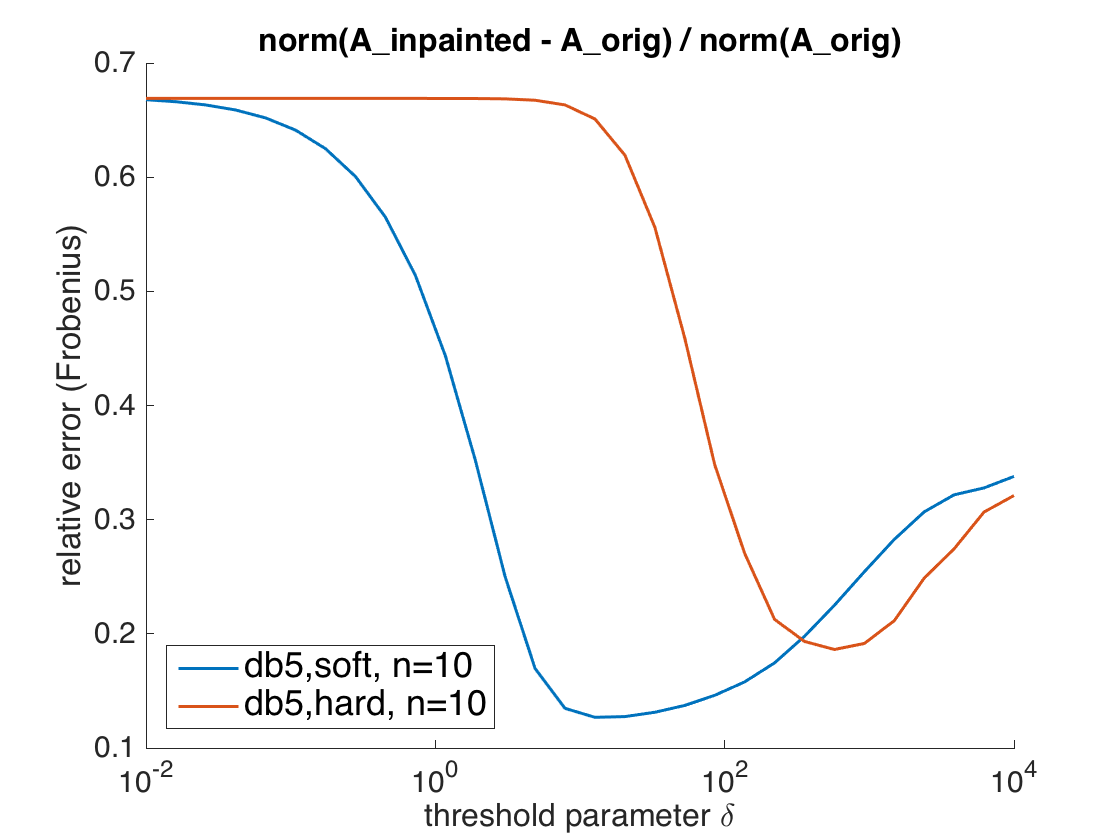
\includegraphics[width=0.8\textwidth]{../src/inpainting/error_plot_3}
    \caption{Het relatieve verschil beschreven \eqref{eq:matti_eq1} in fuctie van de threshold parameter $\delta$ voor zowel soft als hard thresholding. Instellingen algoritme: wavelet: 'db5', level $N = 10$, 50 iteraties voor elke waarde van $\delta$. Het relatieve verschil tussen de onbeschadigde en de beschadige foto is ongeveer $0.67$. De foto van lena overschreven met tekst van in figuur \ref{fig:matti_fig_1e} is gebruikt.}
    \label{fig:matti_error_plot_3}
\end{figure}

\begin{figure}
    \centering
    \begin{subfigure}[b]{0.45\textwidth}
        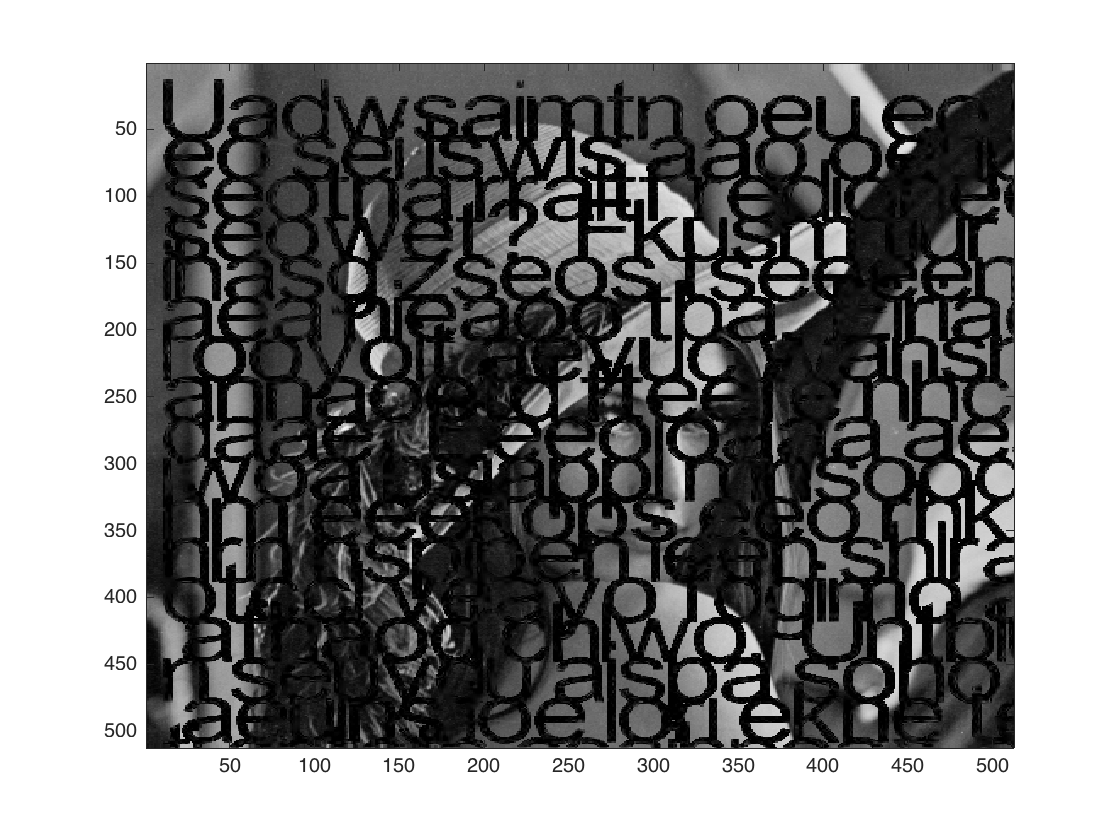
\includegraphics[width=\textwidth]{../src/inpainting/lena_failed_4}
        \caption{ \textbf{Hard thresholding} met te lage waarde van $\mathbf{\delta = 10 }$ . (volgens figuur \ref{fig:matti_error_plot_3})}
        \label{fig:matti_failed_4}
    \end{subfigure}
    ~ %add desired spacing between images, e. g. ~, \quad, \qquad, \hfill etc. 
    %(or a blank line to force the subfigure onto a new line)
    \begin{subfigure}[b]{0.45\textwidth}
        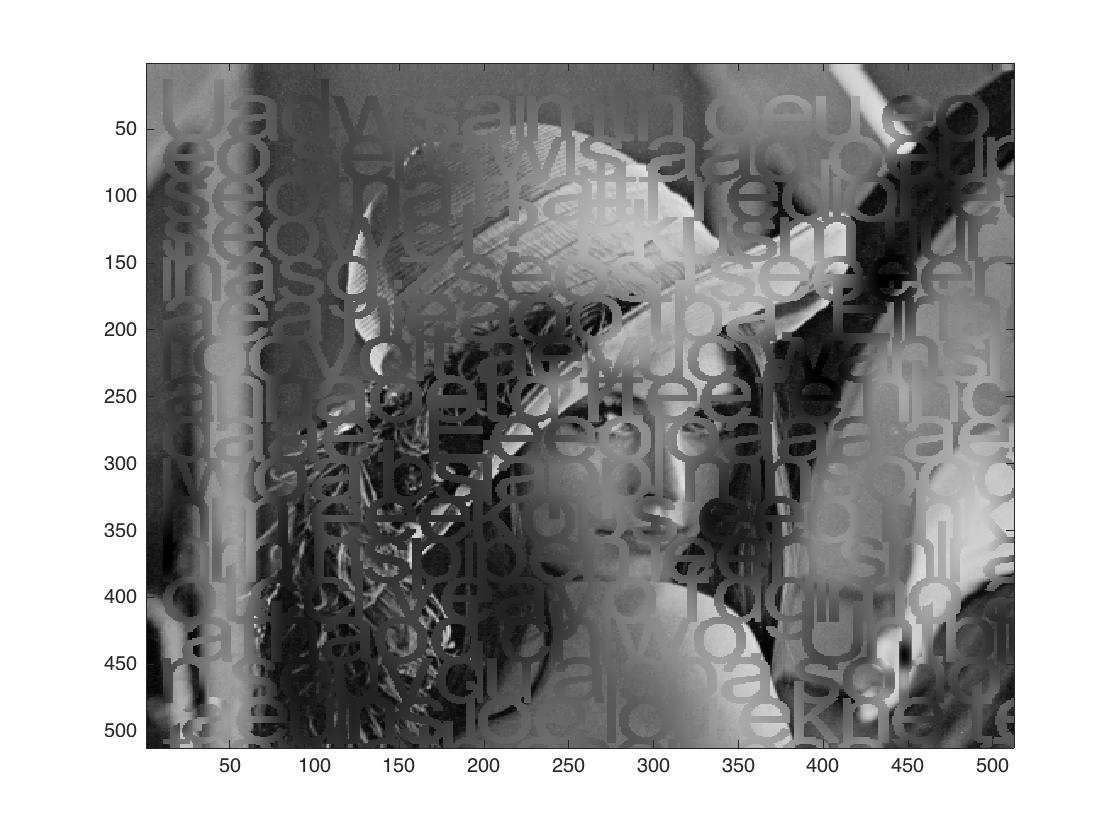
\includegraphics[width=\textwidth]{../src/inpainting/lena_optimal_4}
        \caption{\textbf{Hard thresholding} met de optinale waarde van $\mathbf{\delta = 1000 }$ . (volgens figuur \ref{fig:matti_error_plot_3})}
        \label{fig:matti_optimal_4}
    \end{subfigure}
    \caption{Met tekst overschreven figuur \ref{fig:matti_fig_1e} ingekleurd met 'inpainting' algoritme. Instellingen algoritme: wavelet: 'db5', level $N = 10$, hard thresholding, 200 iteraties. De inkleuring in de linkse figuur is volleding mislukt vanwege een blijkbaar te lage waarde van $\delta$.} \label{fig:matti_hard_4}
\end{figure}

met $A$ de matrix met pixel waarden corresponderend met de foto. In figuur \ref{fig:matti_error_plot_3} kan men duidelijk het verschil zien tussen soft en hard thresholding. Soft thresholding bereikt een lager minimum rond de optimale waarde $\delta = 10$. Het minimum bij hard thresholding ligt iets hoger en wordt bereikt voor veel grotere waarden van $\delta$. Opmerkelijk is dat hard thresholding het heel slecht doet indien de parameter $\delta$ relatief klein in tegenstelling tot soft thresholding. In figuur \ref{fig:matti_hard_4} is hard thresholding gebruikt met een te lage waarde van $\delta$ en de optimale waarde van $\delta$ (minimum rode curve figuur \ref{fig:matti_error_plot_3}). Met $\delta = 10$ mislukt het inkleuren volledig. Dit was te verwachten als we kijken naar figuur \ref{fig:matti_error_plot_3}. Volgens figuur \ref{fig:matti_error_plot_3} zou de optimale waarde van $\delta$ bij hard thresholding rond $1000$ moeten liggen. Hoewel figuur \ref{fig:matti_optimal_4} ($\delta = 1000$)  niet heel slecht is, verkies ik persoonlijk toch figuur \ref{fig:matti_hard_2} ($\delta = 100$) boven figuur \ref{fig:matti_optimal_4} alhoewel het relatieve verschil hierbij minder is. In figuur \ref{fig:matti_optimal_4} zijn nog heel duidelijk de letters te zien. De conclusie is dus dat men niet louter naar het minimale verschil in norm moet kijken maar ook naar het bekomen resultaat. Een tweede conclusie is dat soft thresholding het veel beter doet als hard thresholding voor meer verschillende ordes van $\delta$. Soft thresholding heeft minder last met de randen van de letters in tegenstelling to hard thresholding.



\subsection{Redundant vs non-redundant wavelet transformaties}

In dit hoofdstuk zullen we kort het verschil bestuderen tussen redundant en non-redundant wavelet transformaties.

!!!!!!!!!!! commando iswt2 geeft steeds errors !!!!!!!!!!!!!!!!!!!!!!!!!!!!!!!!!!!!!!!

\subsection{Wavelet types}

In dit hoofdstuk zal kort het verschil in de resultaten tussen verschillende type wavelets besproken worden. In figuur \ref{fig:matti_fig_5} zijn de 'inpainting' resultaten getoond voor 6 verschillende soorten wavelets. De SNR waarden zijn er steeds bij vermeld. In figuur \ref{fig:matti_fig_haar} is de Haar wavelet gebruikt. In deze figuur zijn kleine blokjes te zien, Dit is omdat de Haar wavelet niet geschikt is voor continue overgangen. De corresponderende SNR waarde is $16.19$. De 2 Daubechies wavelets in figuur \ref{fig:matti_fig_db2} en \ref{fig:matti_fig_db6} doen het beter als de haar wavelet. Dit is zowel te zien in de figuur als de SNR waarde. De reden hiervoor is dat Daubechies wavelets beter geschikt zijn voor continue overgangen. In figuur \ref{fig:matti_fig_bior33} is een biorthogonale spline wavelet gebruikt. In deze figuur is een heel slecht resultaat bekomen. De beste resultaten zijn bij de Coiflet en Symlet wavelet in figuur \ref{fig:matti_fig_coif4} en figuur \ref{fig:matti_fig_sym5}.


\begin{figure}
    \centering
    \begin{subfigure}[b]{0.45\textwidth}
        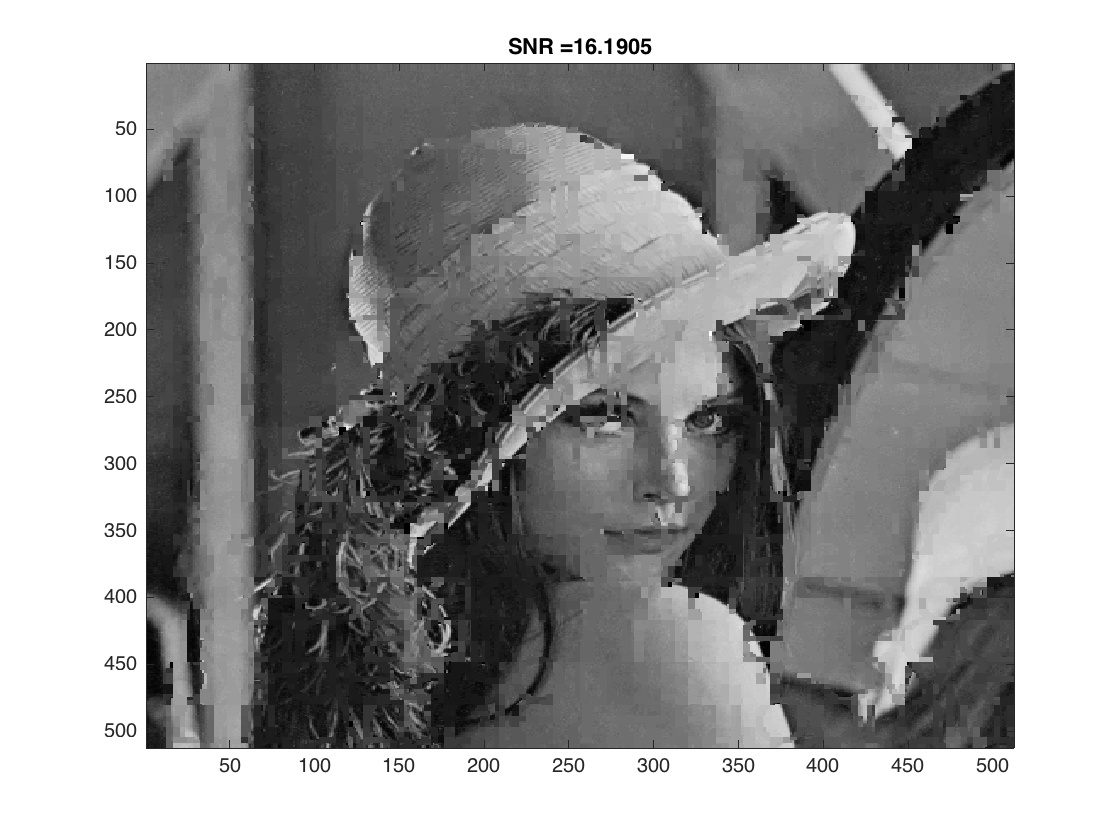
\includegraphics[width=\textwidth]{../src/inpainting/vraag_2_4_haar}
        \caption{\textbf{Haar wavelet, \\ SNR = $\mathbf{16.19}$} }
        \label{fig:matti_fig_haar}
    \end{subfigure}
    ~ %add desired spacing between images, e. g. ~, \quad, \qquad, \hfill etc. 
    %(or a blank line to force the subfigure onto a new line)
    \begin{subfigure}[b]{0.45\textwidth}
        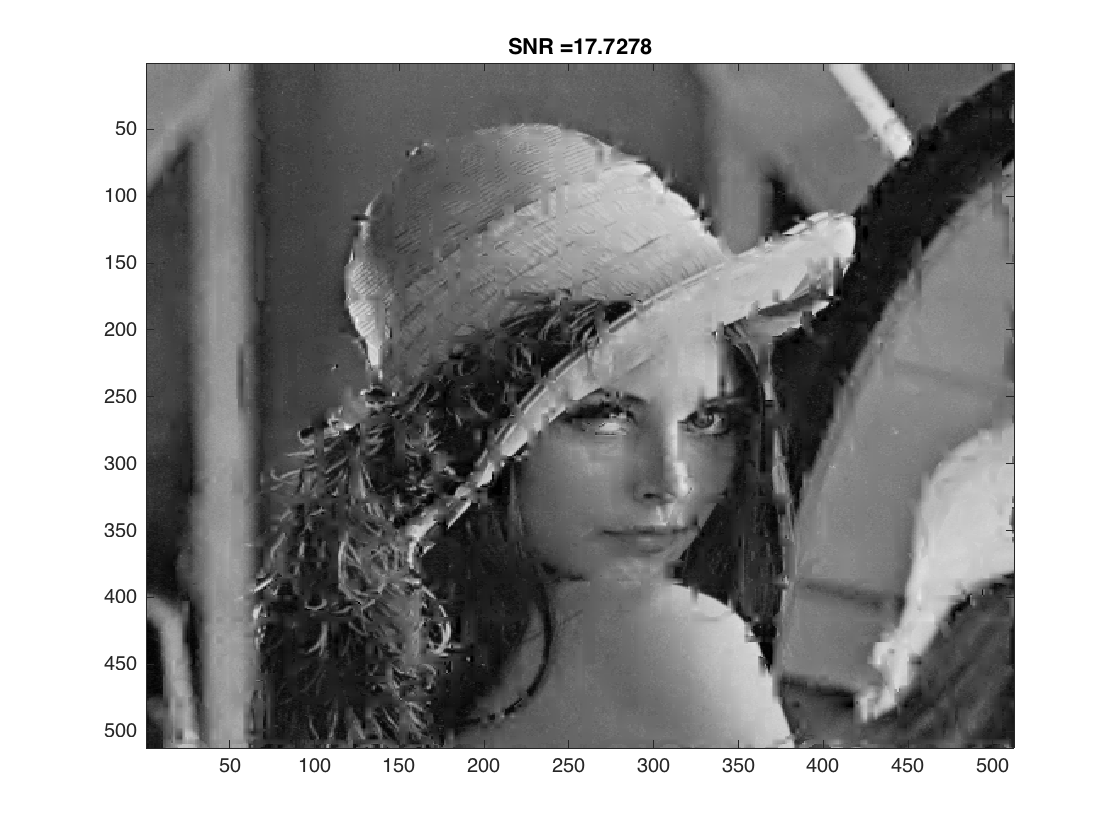
\includegraphics[width=\textwidth]{../src/inpainting/vraag_2_4_db2}
        \caption{\textbf{Daubechies 'db2' wavelet, \\ SNR = $\mathbf{17.73}$} }
        \label{fig:matti_fig_db2}
    \end{subfigure}
    \begin{subfigure}[b]{0.45\textwidth}
        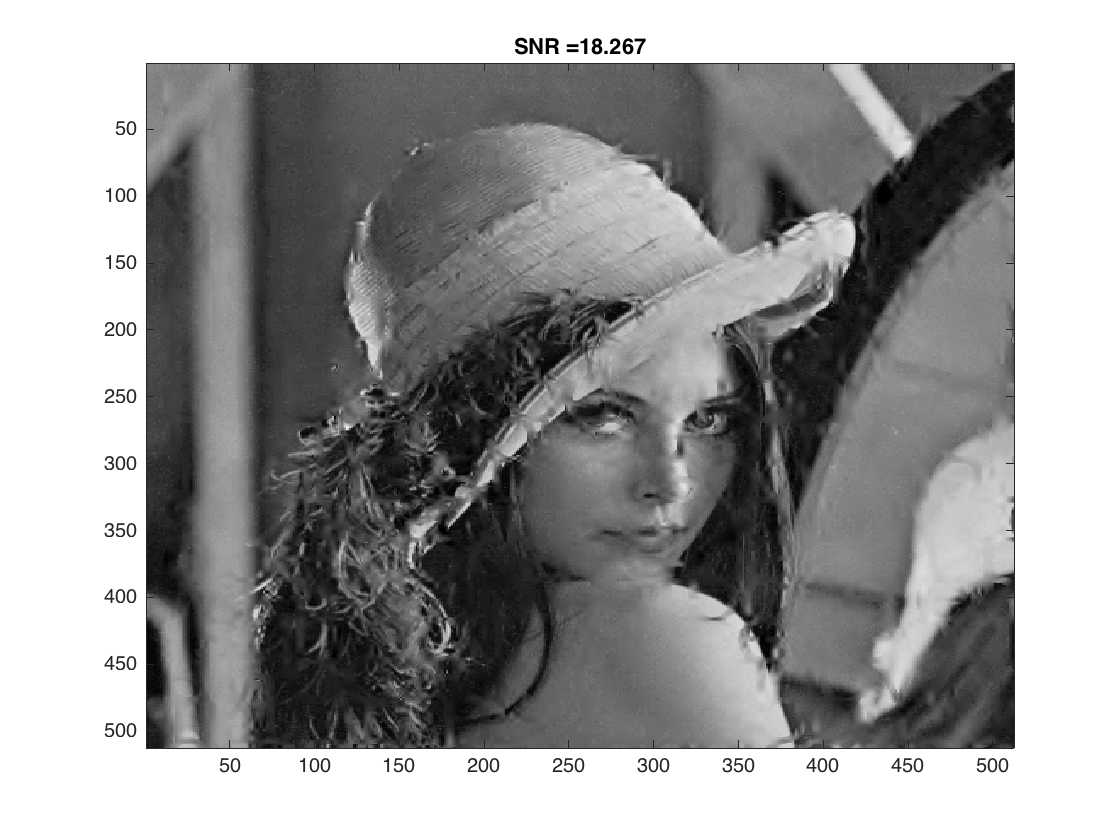
\includegraphics[width=\textwidth]{../src/inpainting/vraag_2_4_db6}
        \caption{\textbf{Daubechies 'db6' wavelet, \\ SNR = $\mathbf{18.26}$} }
        \label{fig:matti_fig_db6}
    \end{subfigure}
    ~ %add desired spacing between images, e. g. ~, \quad, \qquad, \hfill etc. 
    %(or a blank line to force the subfigure onto a new line)
    \begin{subfigure}[b]{0.45\textwidth}
        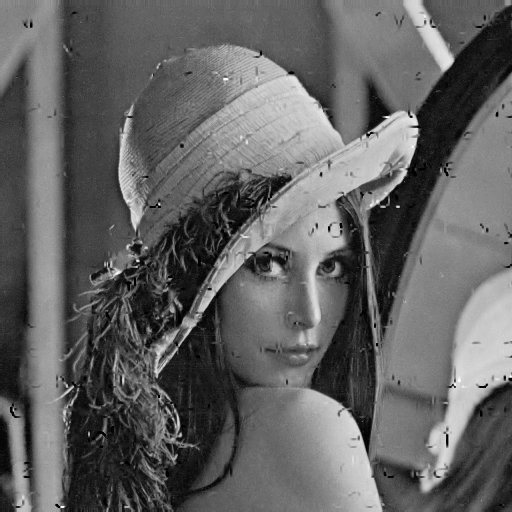
\includegraphics[width=\textwidth]{../src/inpainting/vraag_2_4_bior33}
        \caption{\textbf{ CDF wavelet 'bior3.3', \\ SNR = $\mathbf{11.92}$} }
        \label{fig:matti_fig_bior33}
    \end{subfigure}
        \begin{subfigure}[b]{0.45\textwidth}
        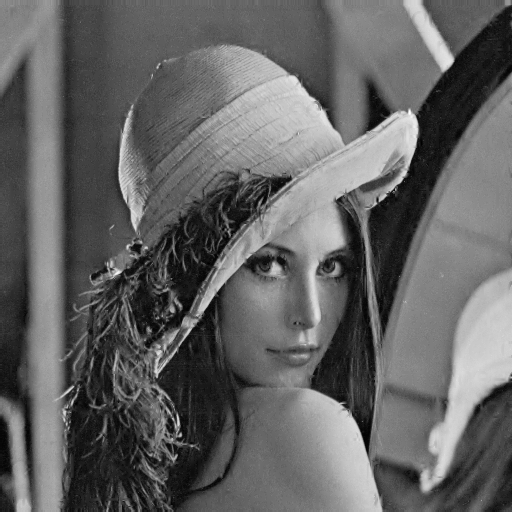
\includegraphics[width=\textwidth]{../src/inpainting/vrag_2_4_coif4}
        \caption{\textbf{ Coiflet wavelet 'coif4', \\ SNR = $\mathbf{18.52}$} }
        \label{fig:matti_fig_coif4}
    \end{subfigure}
    ~ %add desired spacing between images, e. g. ~, \quad, \qquad, \hfill etc. 
    %(or a blank line to force the subfigure onto a new line)
    \begin{subfigure}[b]{0.45\textwidth}
        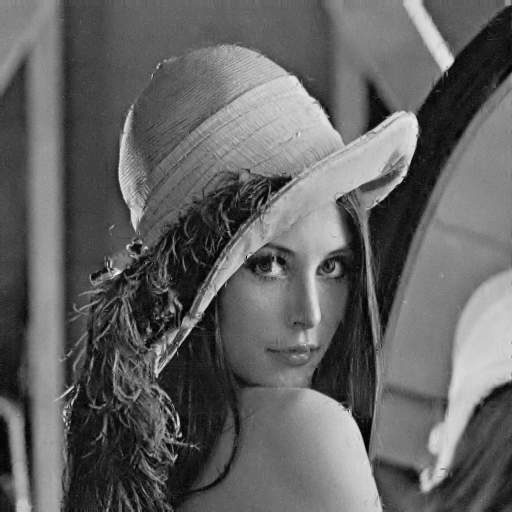
\includegraphics[width=\textwidth]{../src/inpainting/vraag_2_4_sym5}
        \caption{\textbf{ Symlet wavelet 'sym5', \\ SNR = $\mathbf{18.53}$} }
        \label{fig:matti_fig_sym5}
    \end{subfigure}
    \caption{Resultaten van het 'Inpainting' algoritme voor verschillende soorten wavelets. Instellingen algoritme: level $N = 10$, soft thresholding, threshold parameter $\delta = 10$, 200 iteraties.}\label{fig:matti_fig_5}
\end{figure}






















\FloatBarrier

\begin{figure}
    \centering
    \begin{subfigure}[b]{0.45\textwidth}
        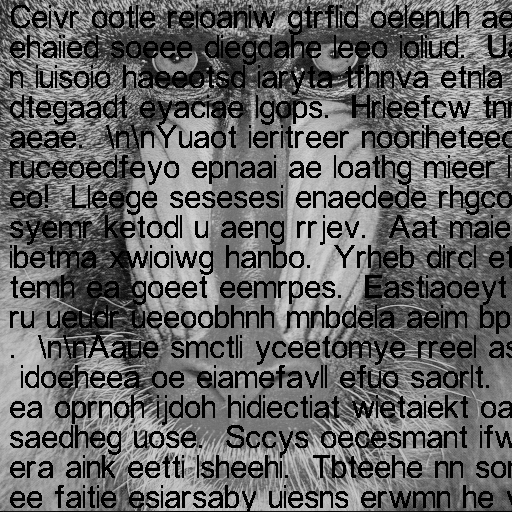
\includegraphics[width=\textwidth]{../src/inpainting/baboon_broke}
        \caption{Met tekst beschadiging}
        \label{fig:tiger}
    \end{subfigure}
    ~ %add desired spacing between images, e. g. ~, \quad, \qquad, \hfill etc. 
    %(or a blank line to force the subfigure onto a new line)
    \begin{subfigure}[b]{0.45\textwidth}
        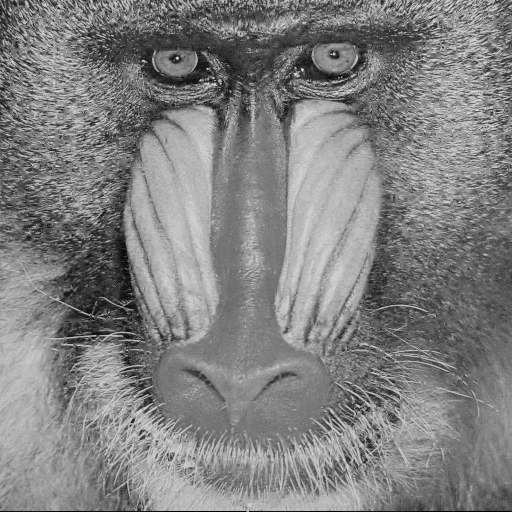
\includegraphics[width=\textwidth]{../src/inpainting/baboon_fixed}
        \caption{Na de reconstructie}
        \label{fig:mouse}
    \end{subfigure}
    \caption{Pictures of lena}\label{fig:baboon}
\end{figure}


\begin{figure}
    \centering
    \begin{subfigure}[b]{0.45\textwidth}
        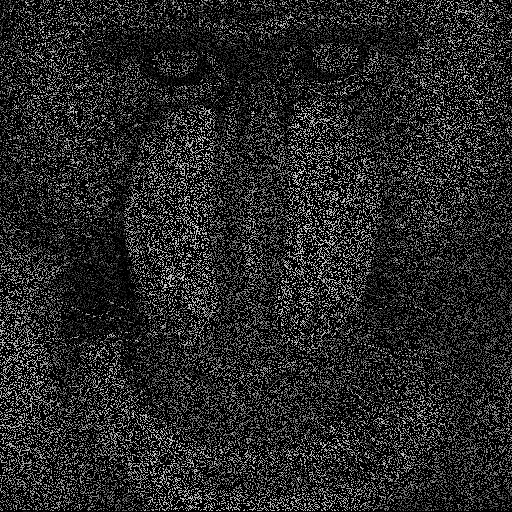
\includegraphics[width=\textwidth]{../src/inpainting/baboon_broke_random}
        \caption{Met random beschadiging (70 procent)}
        \label{fig:tiger}
    \end{subfigure}
    ~ %add desired spacing between images, e. g. ~, \quad, \qquad, \hfill etc. 
    %(or a blank line to force the subfigure onto a new line)
    \begin{subfigure}[b]{0.45\textwidth}
        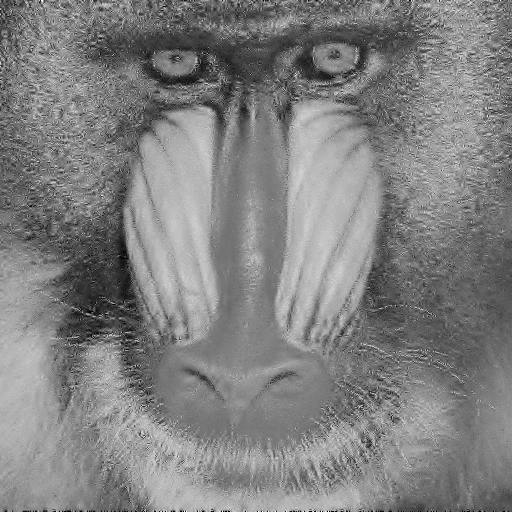
\includegraphics[width=\textwidth]{../src/inpainting/baboon_fixed_random}
        \caption{Na de reconstructie}
        \label{fig:mouse}
    \end{subfigure}
    \caption{Pictures of lena}\label{fig:baboon}
\end{figure}


\begin{figure}
    \centering
    \begin{subfigure}[b]{0.45\textwidth}
        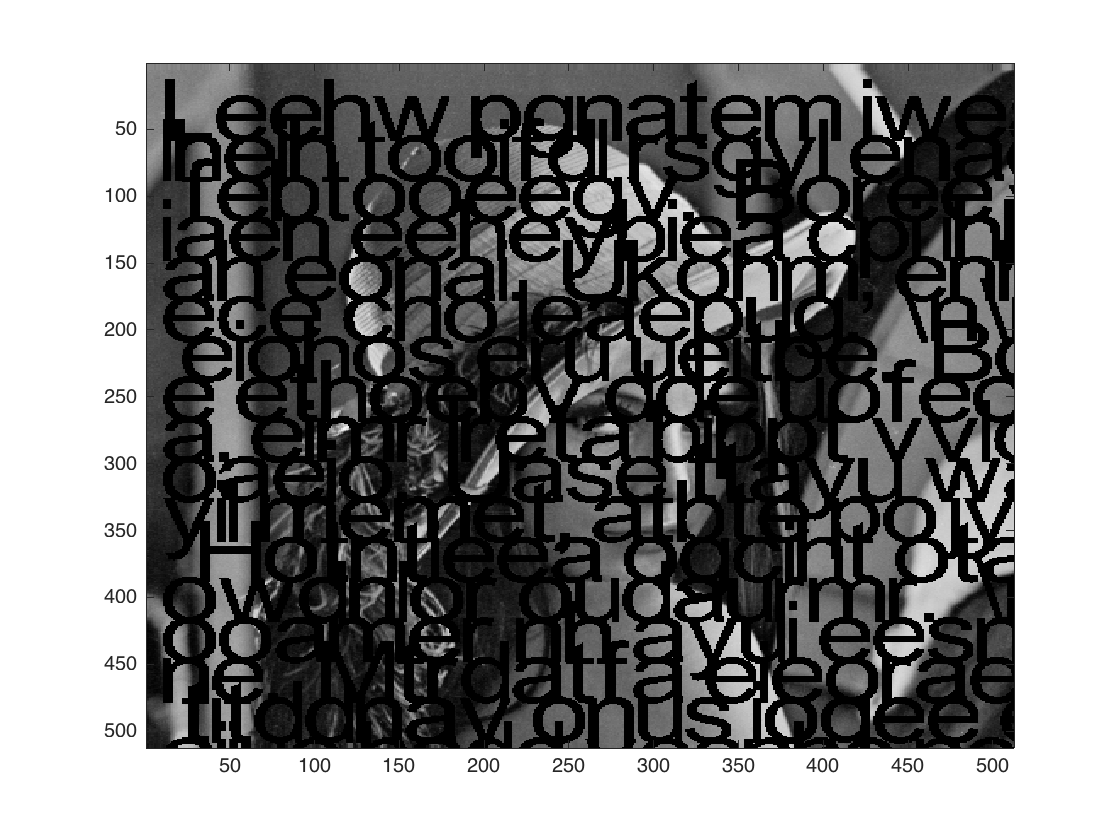
\includegraphics[width=\textwidth]{../src/inpainting/lena_broke2}
        \caption{tekstbeschadigde figuur. \\ \ \\ \ \\ \ \\ \ \\}
        \label{fig:fig1}
    \end{subfigure}
    ~ %add desired spacing between images, e. g. ~, \quad, \qquad, \hfill etc. 
    %(or a blank line to force the subfigure onto a new line)
    \begin{subfigure}[b]{0.45\textwidth}
        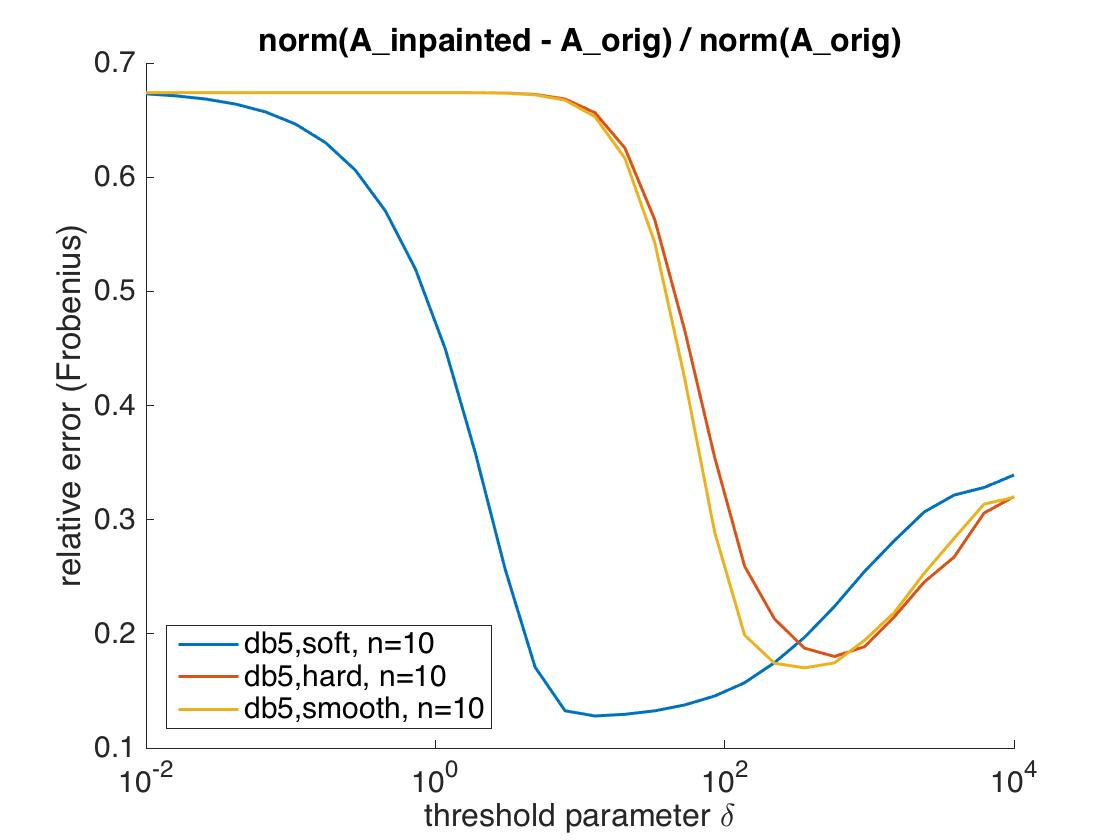
\includegraphics[width=\textwidth]{../src/inpainting/paint_letters_db5_threskinds_it50}
        \caption{Voor verschillende waarden van de threshold parameter $\delta$ is de figuur ingepaint met telkens $50$ iteraties. De relatieve fout t.o.v. de onbeschadigde figuur is telkens berekent.}
        \label{fig:mouse}
    \end{subfigure}
      \begin{subfigure}[b]{0.45\textwidth}
        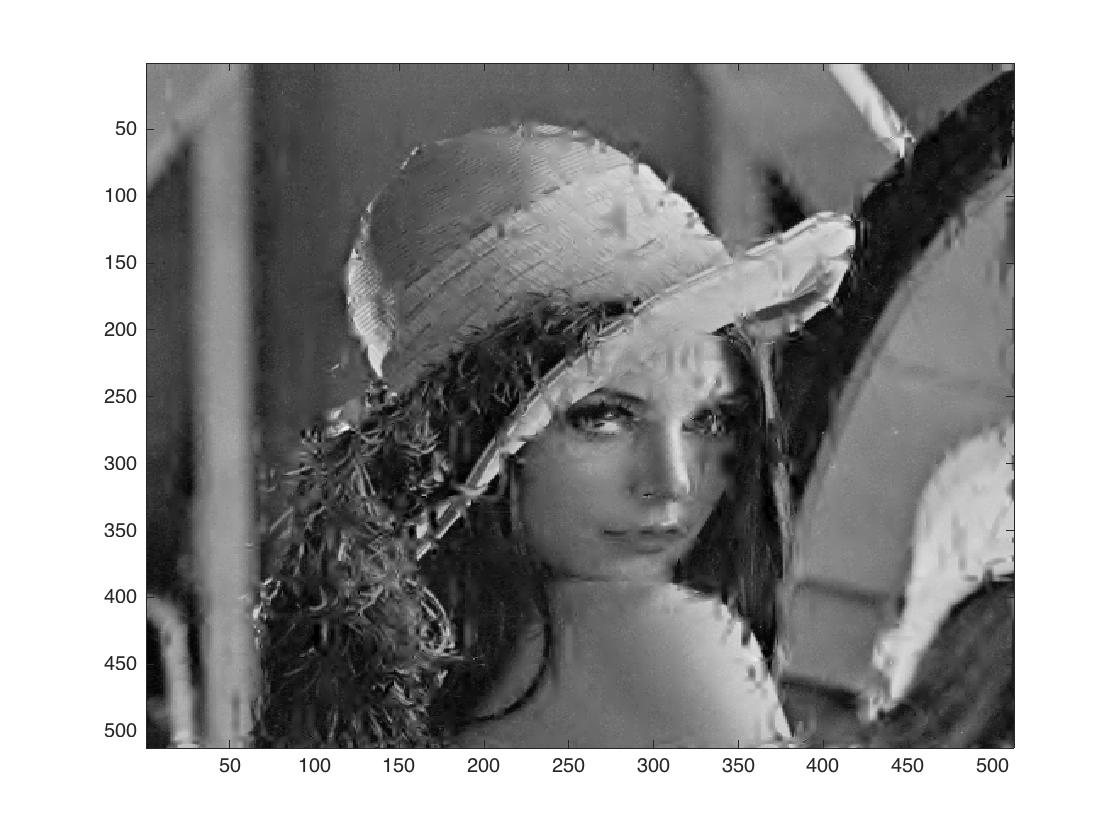
\includegraphics[width=\textwidth]{../src/inpainting/soft_succeed}
        \caption{figuur \ref{fig:fig1} ingepaint met 'db5' wavelets. Soft thresholding is gebruikt met parameter $\delta = 10$. Hier is het goed gelukt, de blauwe curve bereikt zijn mimimum rond $\delta = 10$. \\}
        \label{fig:tiger}
    \end{subfigure}
    ~ %add desired spacing between images, e. g. ~, \quad, \qquad, \hfill etc. 
    %(or a blank line to force the subfigure onto a new line)
    \begin{subfigure}[b]{0.45\textwidth}
        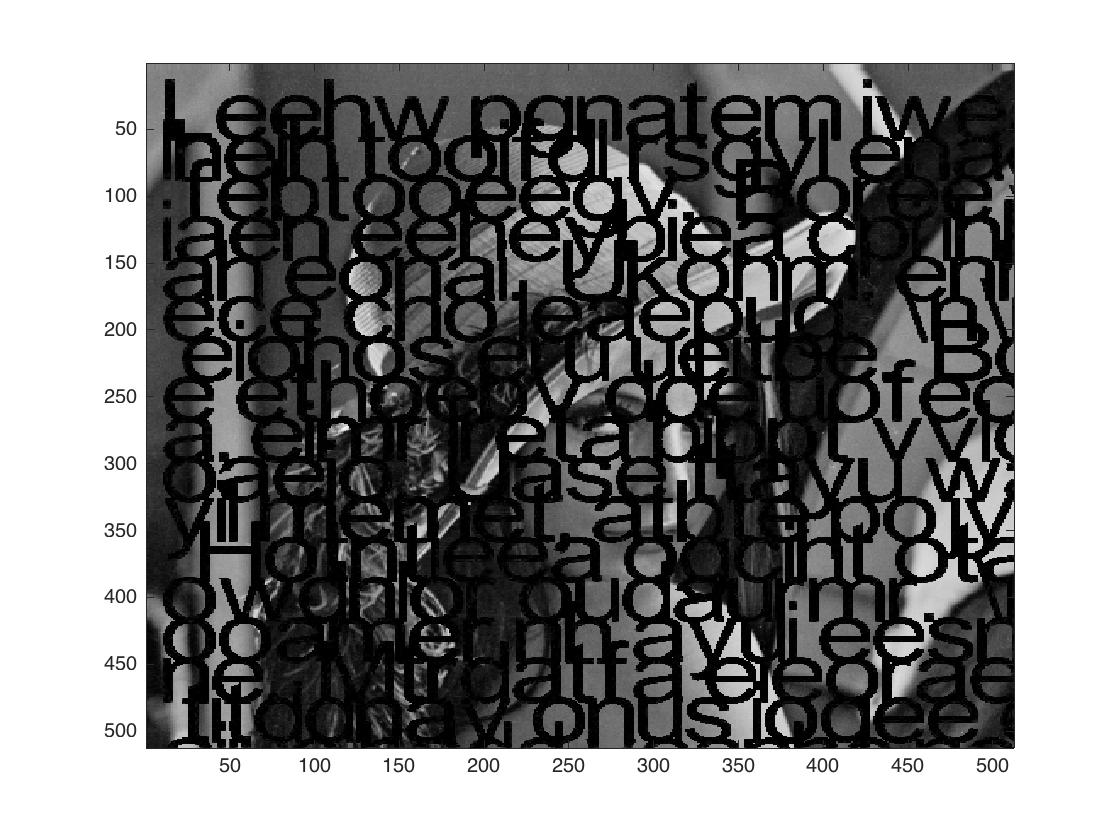
\includegraphics[width=\textwidth]{../src/inpainting/hard_fail}
        \caption{figuur \ref{fig:fig1} ingepaint met 'db5' wavelets. Hard thresholding is gebruikt met parameter $\delta = 10$. Hier is het mislukt. De reden hiervoor is dat de  rode curve voor $\delta = 10$ totaal niet het mimimum bereikt.}
        \label{fig:mouse}
    \end{subfigure}
    \caption{Effect van threshold parameter en threshold techniek bij inpainting}\label{fig:baboon}
\end{figure}

\begin{figure}
    \centering
    \begin{subfigure}[b]{0.7\textwidth}
        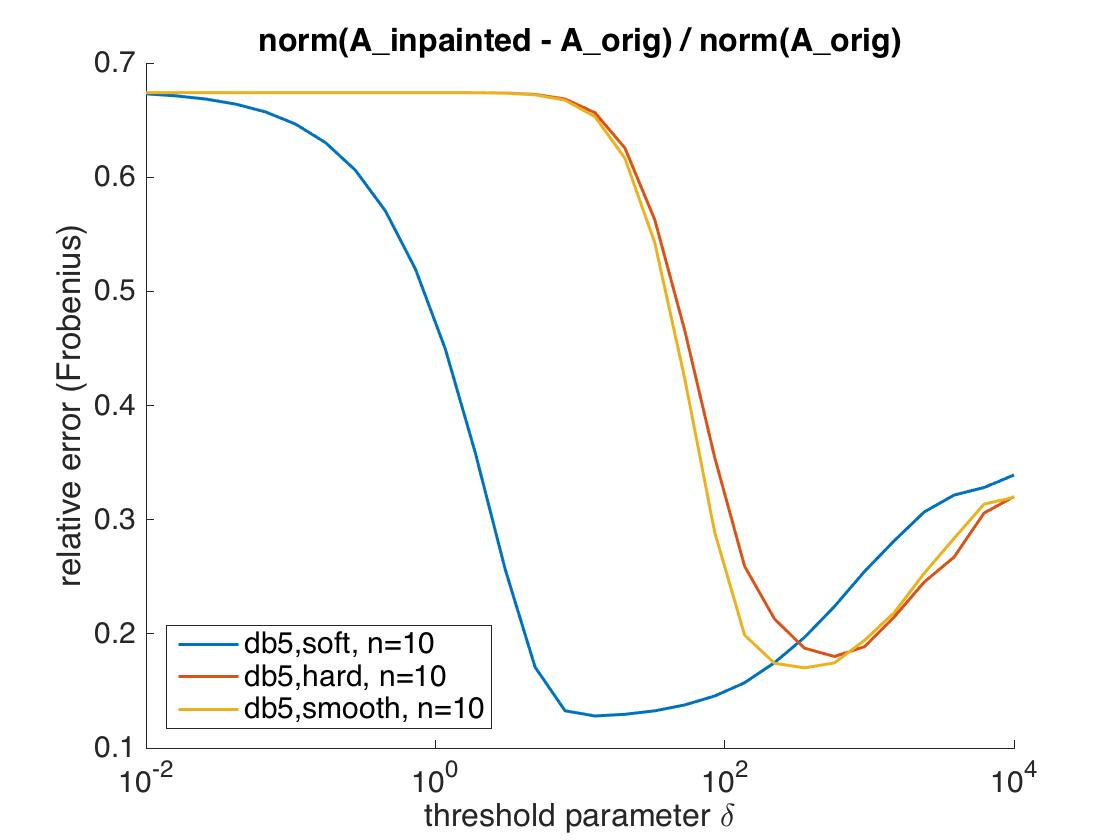
\includegraphics[width=\textwidth]{../src/inpainting/paint_letters_db5_threskinds_it50}
        \caption{Voor verschillende waarden van de threshold parameter $\delta$ is de figuur ingepaint met telkens $50$ iteraties. De relatieve fout t.o.v. de onbeschadigde figuur is telkens berekent. verschillende threshold technieken zijn gebruikt.(dezelfde figuur als vorige pagina)}
        \label{fig:tiger}
    \end{subfigure}
    ~ %add desired spacing between images, e. g. ~, \quad, \qquad, \hfill etc. 
    %(or a blank line to force the subfigure onto a new line)
    \begin{subfigure}[b]{0.7\textwidth}
        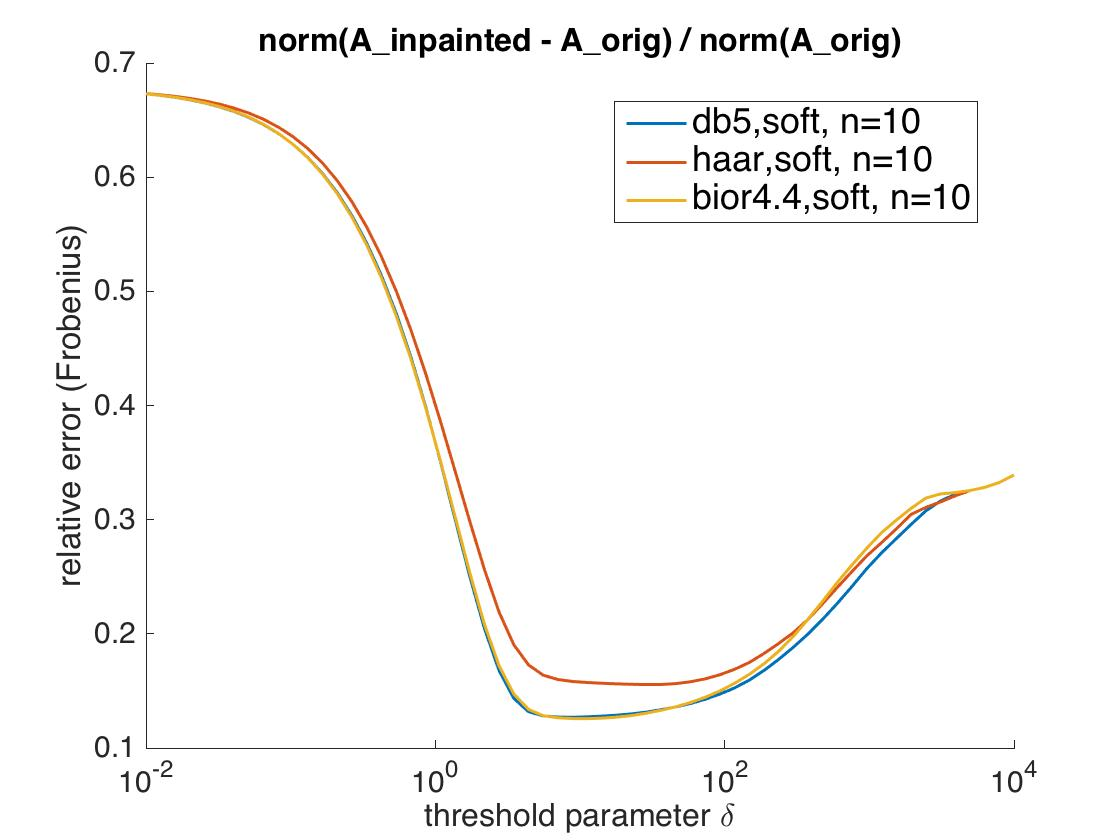
\includegraphics[width=\textwidth]{../src/inpainting/paint_letter_wavekinds_soft_it50}
        \caption{Voor verschillende waarden van de threshold parameter $\delta$ is de figuur ingepaint met telkens $50$ iteraties. De relatieve fout t.o.v. de onbeschadigde figuur is telkens berekent.verschillende soorten wavelets zijn gebruikt.}
        \label{fig:mouse}
    \end{subfigure}
    \caption{plots error vs $\delta$}\label{fig:baboon}
\end{figure}


\begin{figure}
    \centering
    \begin{subfigure}[b]{0.7\textwidth}
        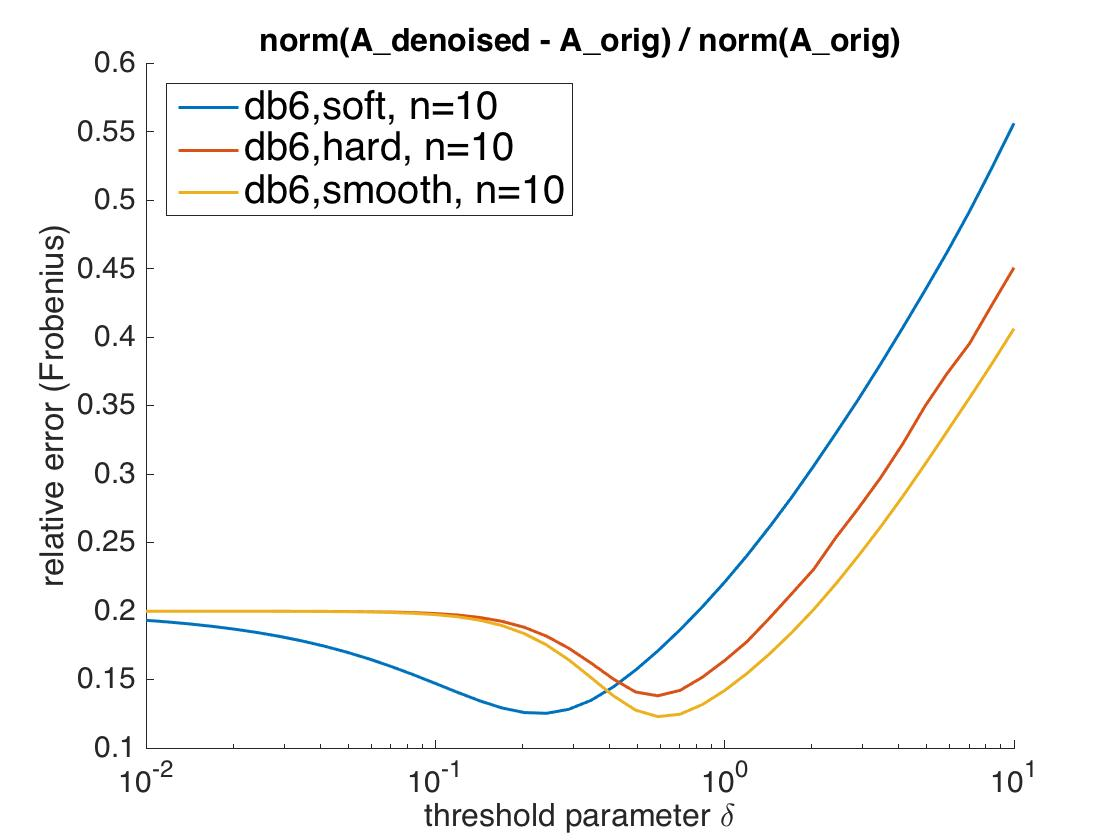
\includegraphics[width=\textwidth]{../src/denoising/denoised_err_threskinds}
        \caption{Voor verschillende waarden van de threshold parameter $\delta$ is een noisy figuur gedenoised. De relatieve fout t.o.v. de originele figuur(zonder noise) is telkens berekent. verschillende threshold technieken zijn gebruikt. De onbewerkte noisy figuur heeft een relatieve fout van $0.2$. Conclusie: opletten met de waarde van de threshold parameter.}
        \label{fig:tiger}
    \end{subfigure}
    ~ %add desired spacing between images, e. g. ~, \quad, \qquad, \hfill etc. 
    %(or a blank line to force the subfigure onto a new line)
    \begin{subfigure}[b]{0.7\textwidth}
        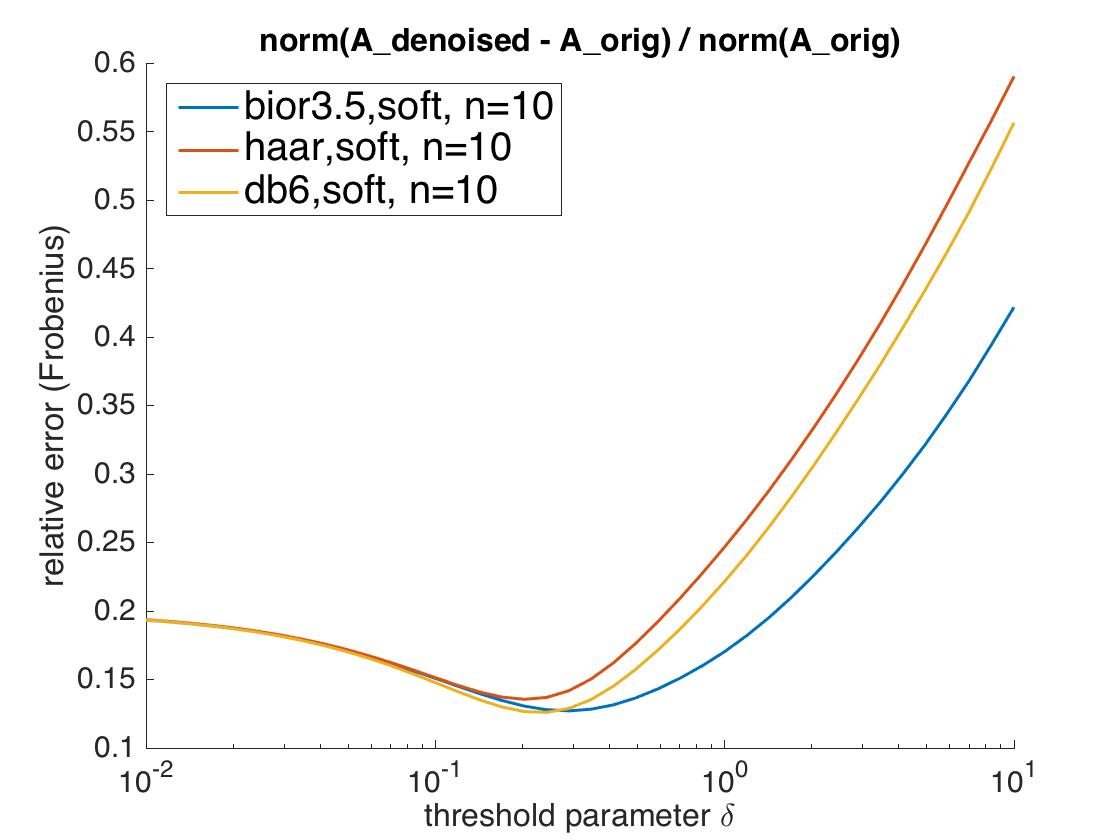
\includegraphics[width=\textwidth]{../src/denoising/denoised_err_wavekinds}
        \caption{Voor verschillende waarden van de threshold parameter $\delta$ is een noisy figuur gedenoised. De relatieve fout t.o.v. de originele figuur(zonder noise) is telkens berekent. De onbewerkte noisy figuur heeft een relatieve fout van $0.2$.verschillende soorten wavelets zijn gebruikt. Conclusie: opletten met de waarde van de threshold parameter..}
        \label{fig:mouse}
    \end{subfigure}
    \caption{plots error vs $\delta$}\label{fig:baboon}
\end{figure}

\end{document}
